%!TeX TS-program = pdflatex
%!TeX encoding = UTF-8 Unicode
%!TeX spellcheck = en-US
%!BIB TS-program = bibtex
% -*- coding: UTF-8; -*-
% vim: set fenc=utf-8
%TODO include changing point theory and bibliography
%%%%%%%%%%%%%%%%%%%%%%%%%%%%%%%%%%%%%%%%%%%%%%%%%%%%%%%%%%%%%%%%%%%%%
\newcommand{\AuthorA}{Chlo\'e Pasturel}
\newcommand{\AuthorB}{Anna Montagnini}%
\newcommand{\AuthorC}{Laurent U.~Perrinet}%
\newcommand{\Address}{Institut de Neurosciences de la Timone, CNRS / Aix-Marseille Universit\'e - Marseille, France}%
\newcommand{\Website}{http://invibe.net/LaurentPerrinet}%
\newcommand{\Email}{Laurent.Perrinet@univ-amu.fr}%
\newcommand{\Title}{Anticipating a dynamic, switching probabilistic bias in visual motion direction}
\newcommand{\Acknowledgments}{ANR grant <<Reinforcement and Eye Movements>> \textbf{ANR-13-APPR-0008-02} - code and material @ \url{\Website/Publications/Pasturel_etal2018} }
\newcommand{\Abstract}{
The brain has to constantly adapt to changes in the environment, for instance when a contextual variable switched its state.
For an agent interacting with such an environment, it is important for him to respond to such switches with the shortest delay.
However, this operation has in general to be done with perturbed sensory inputs and solely based on the information available at the present time.
Here, we tested the ability of humans observers, to respond to such random sequences with contextual blocks random length using a known marker for anticipatory responses in smooth pursuit eye movements.
These results were compared to that of a probabilistic agent optimized with respect to this switching model.
We found a good fit of the behaviorally observed anticipatory response compared with other models such as the forgetful model.
Moreover, we could also fit the level of confidence given by human observers with that provided by the model. 
Such results provide a novel method to more generically test cognitive abilities in humans and provide evidence that human observers may represent an anticipatory belief along with its precision.
}
%%%%%%%%%%%%%%%%%%%%%%%%%%%%%%%%%%%%%%%%%%
\documentclass[profile,final,english, draft]{article}%
\usepackage{babel}
% MATHS (AMS)
\usepackage{amsmath}
\usepackage{amsfonts} 
\usepackage{amssymb}
\usepackage{amsthm}
\newcommand{\KL}[2]{\text{KL}( #1 | #2 )}
%% parenthesis
\newcommand{\pa}[1]{\left( #1 \right)}
\newcommand{\bpa}[1]{\big( #1 \big)}
\newcommand{\choice}[1]{ %
	\left\{ %
		\begin{array}{l} #1 \end{array} %
	\right. }
% ensembles
\newcommand{\ens}[1]{ \{ #1 \} }
\newcommand{\enscond}[2]{ \left\{ #1 \;;\; #2 \right\} }
% egal par définition
\newcommand{\eqdef}{\ensuremath{\stackrel{\mbox{\upshape\tiny def.}}{=}}}
\newcommand{\eqset}{\ensuremath{\stackrel{\mbox{\upshape\tiny set}}{=}}}
\newcommand{\eq}[1]{\begin{equation*}#1\end{equation*}}
\newcommand{\eql}[1]{\begin{equation}#1\end{equation}}

\DeclareMathOperator{\argmin}{argmin}
\DeclareMathOperator{\argmax}{argmax}
\newcommand{\uargmin}[1]{\underset{#1}{\argmin}\;}
\newcommand{\uargmax}[1]{\underset{#1}{\argmax}\;}
\newcommand{\umin}[1]{\underset{#1}{\min}\;}
\newcommand{\umax}[1]{\underset{#1}{\max}\;}
\newcommand{\usup}[1]{\underset{#1}{\sup}\;}
% for units
\usepackage{siunitx}%
\newcommand{\ms}{\si{\milli\second}}%

%% Symboles arrondis
\newcommand{\Aa}{\mathcal{A}}
\newcommand{\Bb}{\mathcal{B}}
\newcommand{\Cc}{\mathcal{C}}
\newcommand{\Dd}{\mathcal{D}}
\newcommand{\Ee}{\mathcal{E}}
\newcommand{\Ff}{\mathcal{F}}
\newcommand{\Gg}{\mathcal{G}}
\newcommand{\Hh}{\mathcal{H}}
\newcommand{\Ii}{\mathcal{I}}
\newcommand{\Jj}{\mathcal{J}}
\newcommand{\Kk}{\mathcal{K}}
\newcommand{\Ll}{\mathcal{L}}
\newcommand{\Mm}{\mathcal{M}}
\newcommand{\Nn}{\mathcal{N}}
\newcommand{\Oo}{\mathcal{O}}
\newcommand{\Pp}{\mathcal{P}}
\newcommand{\Qq}{\mathcal{Q}}
\newcommand{\Rr}{\mathcal{R}}
\newcommand{\Ss}{\mathcal{S}}
\newcommand{\Tt}{\mathcal{T}}
\newcommand{\Uu}{\mathcal{U}}
\newcommand{\Vv}{\mathcal{V}}
\newcommand{\Ww}{\mathcal{W}}
\newcommand{\Xx}{\mathcal{X}}
\newcommand{\Yy}{\mathcal{Y}}
\newcommand{\Zz}{\mathcal{Z}}
%% ========  polices de caracteres =============
\usepackage[T1]{fontenc}% 
\usepackage{lmodern}%
\usepackage{t1enc}
\usepackage{ragged2e}
%============ graphics ===================
\usepackage[pdftex]{graphicx}% 
\DeclareGraphicsExtensions{.pdf,.png,.jpg}%
\graphicspath{{./figures/}}%
%\usepackage[numbers,comma,sort&compress,round]{natbib} %
\usepackage[%style=nature,
maxcitenames=2,
maxnames = 2,
firstinits=true,
uniquename=init,
sorting=none,
url=false,
isbn=false,
eprint=false,
texencoding=latin1,
bibencoding=utf8,
autocite=superscript,
backend=bibtex,
%articletitle=false
]{biblatex}%
\addbibresource{Pasturel_etal2018.bib}%
\newcommand{\citep}[1]{(\cite{#1})}
%\newcommand{\citet}[1]{(\textcite{#1})}
%%%%%%%%%%%%%%%%%%%%%%%%%%%%%%
%% OPTIONAL MACRO FILES
%\usepackage{tikz,tkz-euclide} \usetkzobj{all} % loading all objects
%\usetikzlibrary{positioning} \usetikzlibrary{calc}
%\usepackage{sfmath}
%============ hyperref ===================
\usepackage[unicode,linkcolor=red,citecolor=red,filecolor=black,urlcolor=red,pdfborder={0 0 0}]{hyperref}%
\hypersetup{%
pdftitle={\Title},%
pdfauthor={\AuthorA},%< \Email > \Address},%
}%
\usepackage{color}%
%%%%%%%%%%%%%%%%%%%%%%%%%%%%%%%%%%%
\title{\Title}%
\author{\AuthorA, 
%\AuthorB,  
\AuthorC,  \AuthorD\thanks{\Address} }

%%%%%%%%%%%% Her begynner selve dokumentet %%%%%%%%%%%%%%%
\begin{document}%
\maketitle%
%%%%%%%%%%%%%%%%%%%%%%%%%%%%%%%%%%%%%%%%%%%%%%%%%%%%%%%%%%%%%%%%
% Abstract
\begin{abstract}
\Abstract
\end{abstract}

\section{Motivation}

Humans are able to accurately track a moving object with a combination of saccades and smooth eye movements. These movements allow us to align and stabilize the object on the fovea, thus enabling high-resolution visual detection. When predictive information is available about target motion, anticipatory smooth pursuit eye movements (aSPEM) are efficiently generated before target appearance, which reduce the typical sensorimotor delay between target motion onset and foveation. It is generally assumed that the role of anticipatory eye movements is to limit the behavioral impairment due to eye-to-target position and velocity mismatch.

Humans are able to accurately track a moving object with a combination of saccades and smooth eye movements. These movements allow us to align and stabilize the object on the fovea, thus enabling high-resolution visual analysis. When predictive information is available about target motion, anticipatory smooth pursuit eye movements (aSPEM) are efficiently generated before target appearance, which reduce the typical sensorimotor delay between target motion onset and foveation. It is generally assumed that the role of anticipatory eye movements is to limit the behavioral impairment due to eye-to-target position and velocity mismatch.



By manipulating the probability for target motion direction we were able to bias the direction and mean velocity of aSPEM, as measured during a fixed duration gap before target ramp-motion onset. This suggests that probabilistic information may be used to inform the internal representation of motion prediction for the initiation of anticipatory movements~\parencite{Montagnini2010}.



By manipulating the probability for target motion direction, we were able to bias the direction and mean velocity of aSPEM, as measured during a fixed duration gap before target ramp- motion onset. This suggests that probabilistic information may be used to inform the internal representation of motion prediction for the initiation of anticipatory movements. However, such estimate may become particularly challenging in a dynamic context, where the probabilistic contingencies vary in time in an unpredictable way. In addition, whether and how the information processing underlying the buildup of aSPEM is linked to an explicit estimate of probabilities is unknown. We developed a new paired-task paradigm in order to address these two questions. In a first session, participants observe a target moving horizontally with constant speed from the center either to the right or left across trials. The probability of either motion direction changes randomly in time. Participants are asked to estimate "how much they are confident that the target will move to the right or left in the next trial" and to adjust the cursor's position on the screen accordingly. In a second session the participants eye movements are recorded during the observation of the same sequence of random-direction trials.
In parallel, we are developing new automatic routines for the advanced analysis of oculomotor traces. In order to extract the relevant parameters of the oculomotor responses (latency, gain, initial acceleration, catch-up saccades), we developed new tools based on best-fitting procedure of predefined patterns (i.e. the typical smooth pursuit velocity profile).


Throughout the first experimental condition we investigated the integration of environmental statistical regularities in a smooth tracking task with a family of direction-biases for the target motion. What we found was a global and robust effect of direction-bias on anticipatory smooth pursuit. These results are coherent with previous oculomotor findings by our and also other groups (Montagnini et al. 2010; Santos \& Kowler 2017). Typically, aSPEM is observed after a temporal cue and ahead of target motion onset (Kowler and Steinman, 1979a,b, 1984). Some now classical experiments have demonstrated the existence of prediction-based smooth pursuit during the transient disappearance of a moving target (Badler, 2006; Becker \& Fuchs, 1985). Overall, it is now clear that smooth pursuit behavior can be modulated even in the absence of online sensory stimulation. aSPEM were here the core of our research because we wanted to study the trial-by-trial evolution of expectancy-based oculomotor behavior, as well as how sensorimotor expectancy interacts with reward contingencies in shaping oculomotor behavior without direct sensory feedback. In a previous study, (Souto, Montagnini \& Masson, 2008b; Montagnini et al., 2010) we have analyzed how forthcoming motion properties, such as target speed or direction, can be predicted and anticipated with coherent orienting eye movements. We found a graded effect of both the speed and the direction-bias, with mean anticipatory eye velocity linearly related to the probability of motion’s speed or direction. Here, we replicated part of those results using a limited number of direction probability bias and strengthened them by generalizing them on seventeen participants. These results imply that the probability bias over a target’s direction is one additional factor beyond other physical and cognitive cues (Kowler et al, 2014; Santos \& Kowler 2017) that modulate the common predictive framework driving anticipatory behavior to optimize a rapid and precise foveation of the target on its most expected future path. 

%-------------------------------------------------------------%
%: fig:intro
\begin{figure}%[b!]
%\begin{center}
%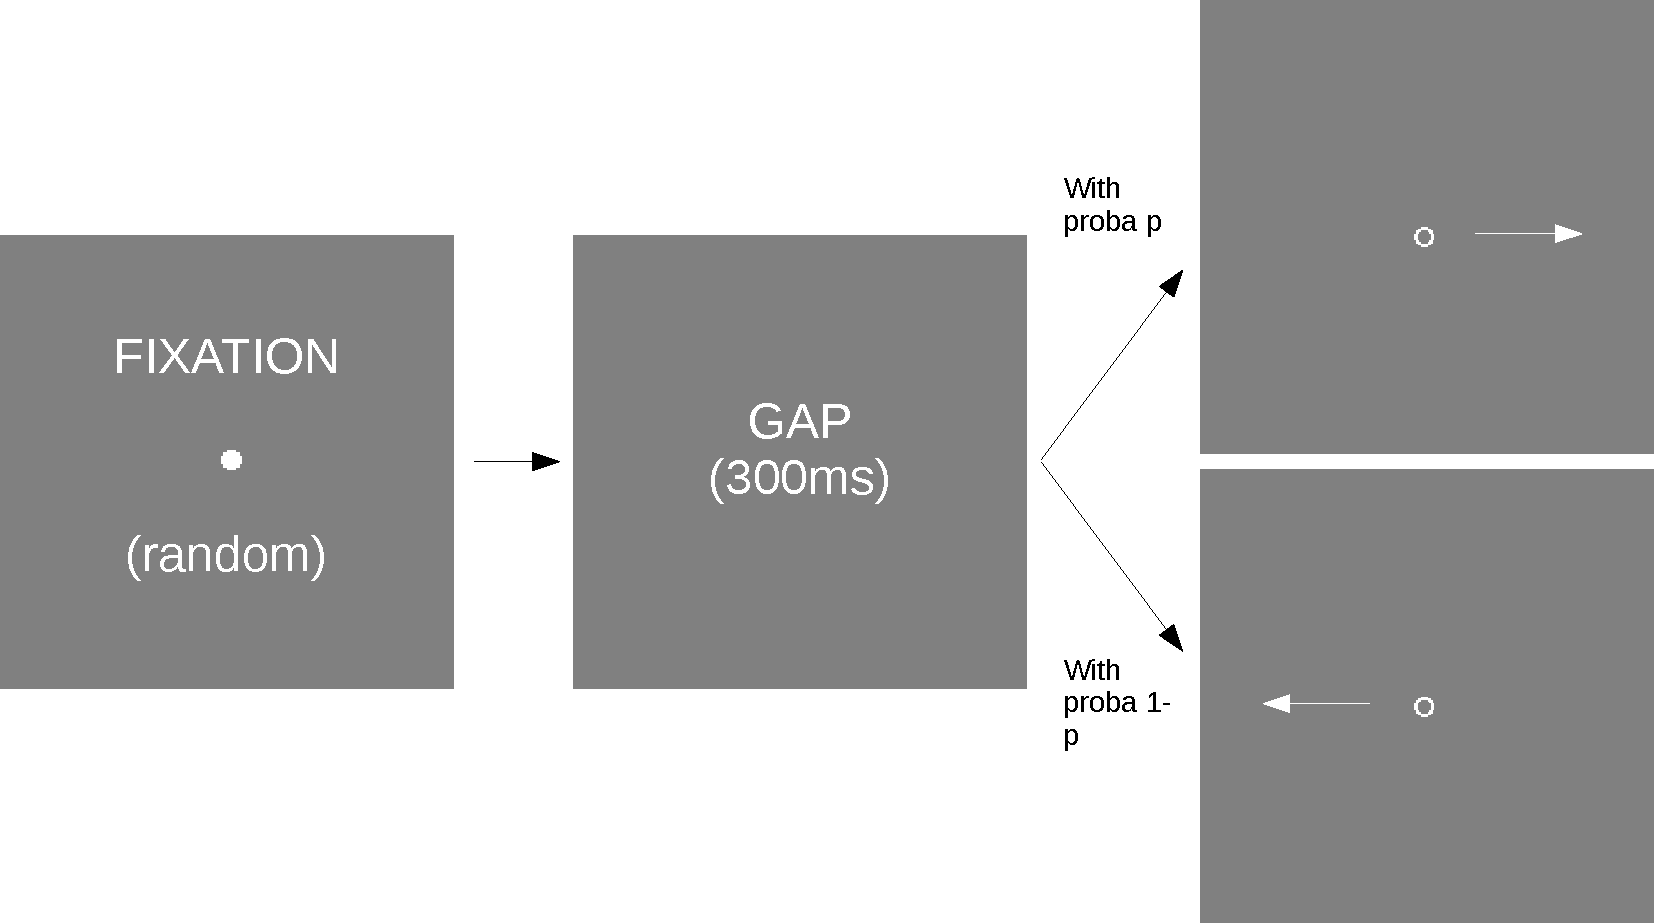
\includegraphics[width=1\linewidth]{anna_methode}
%\end{center}
\begin{tabular}{cc} 
    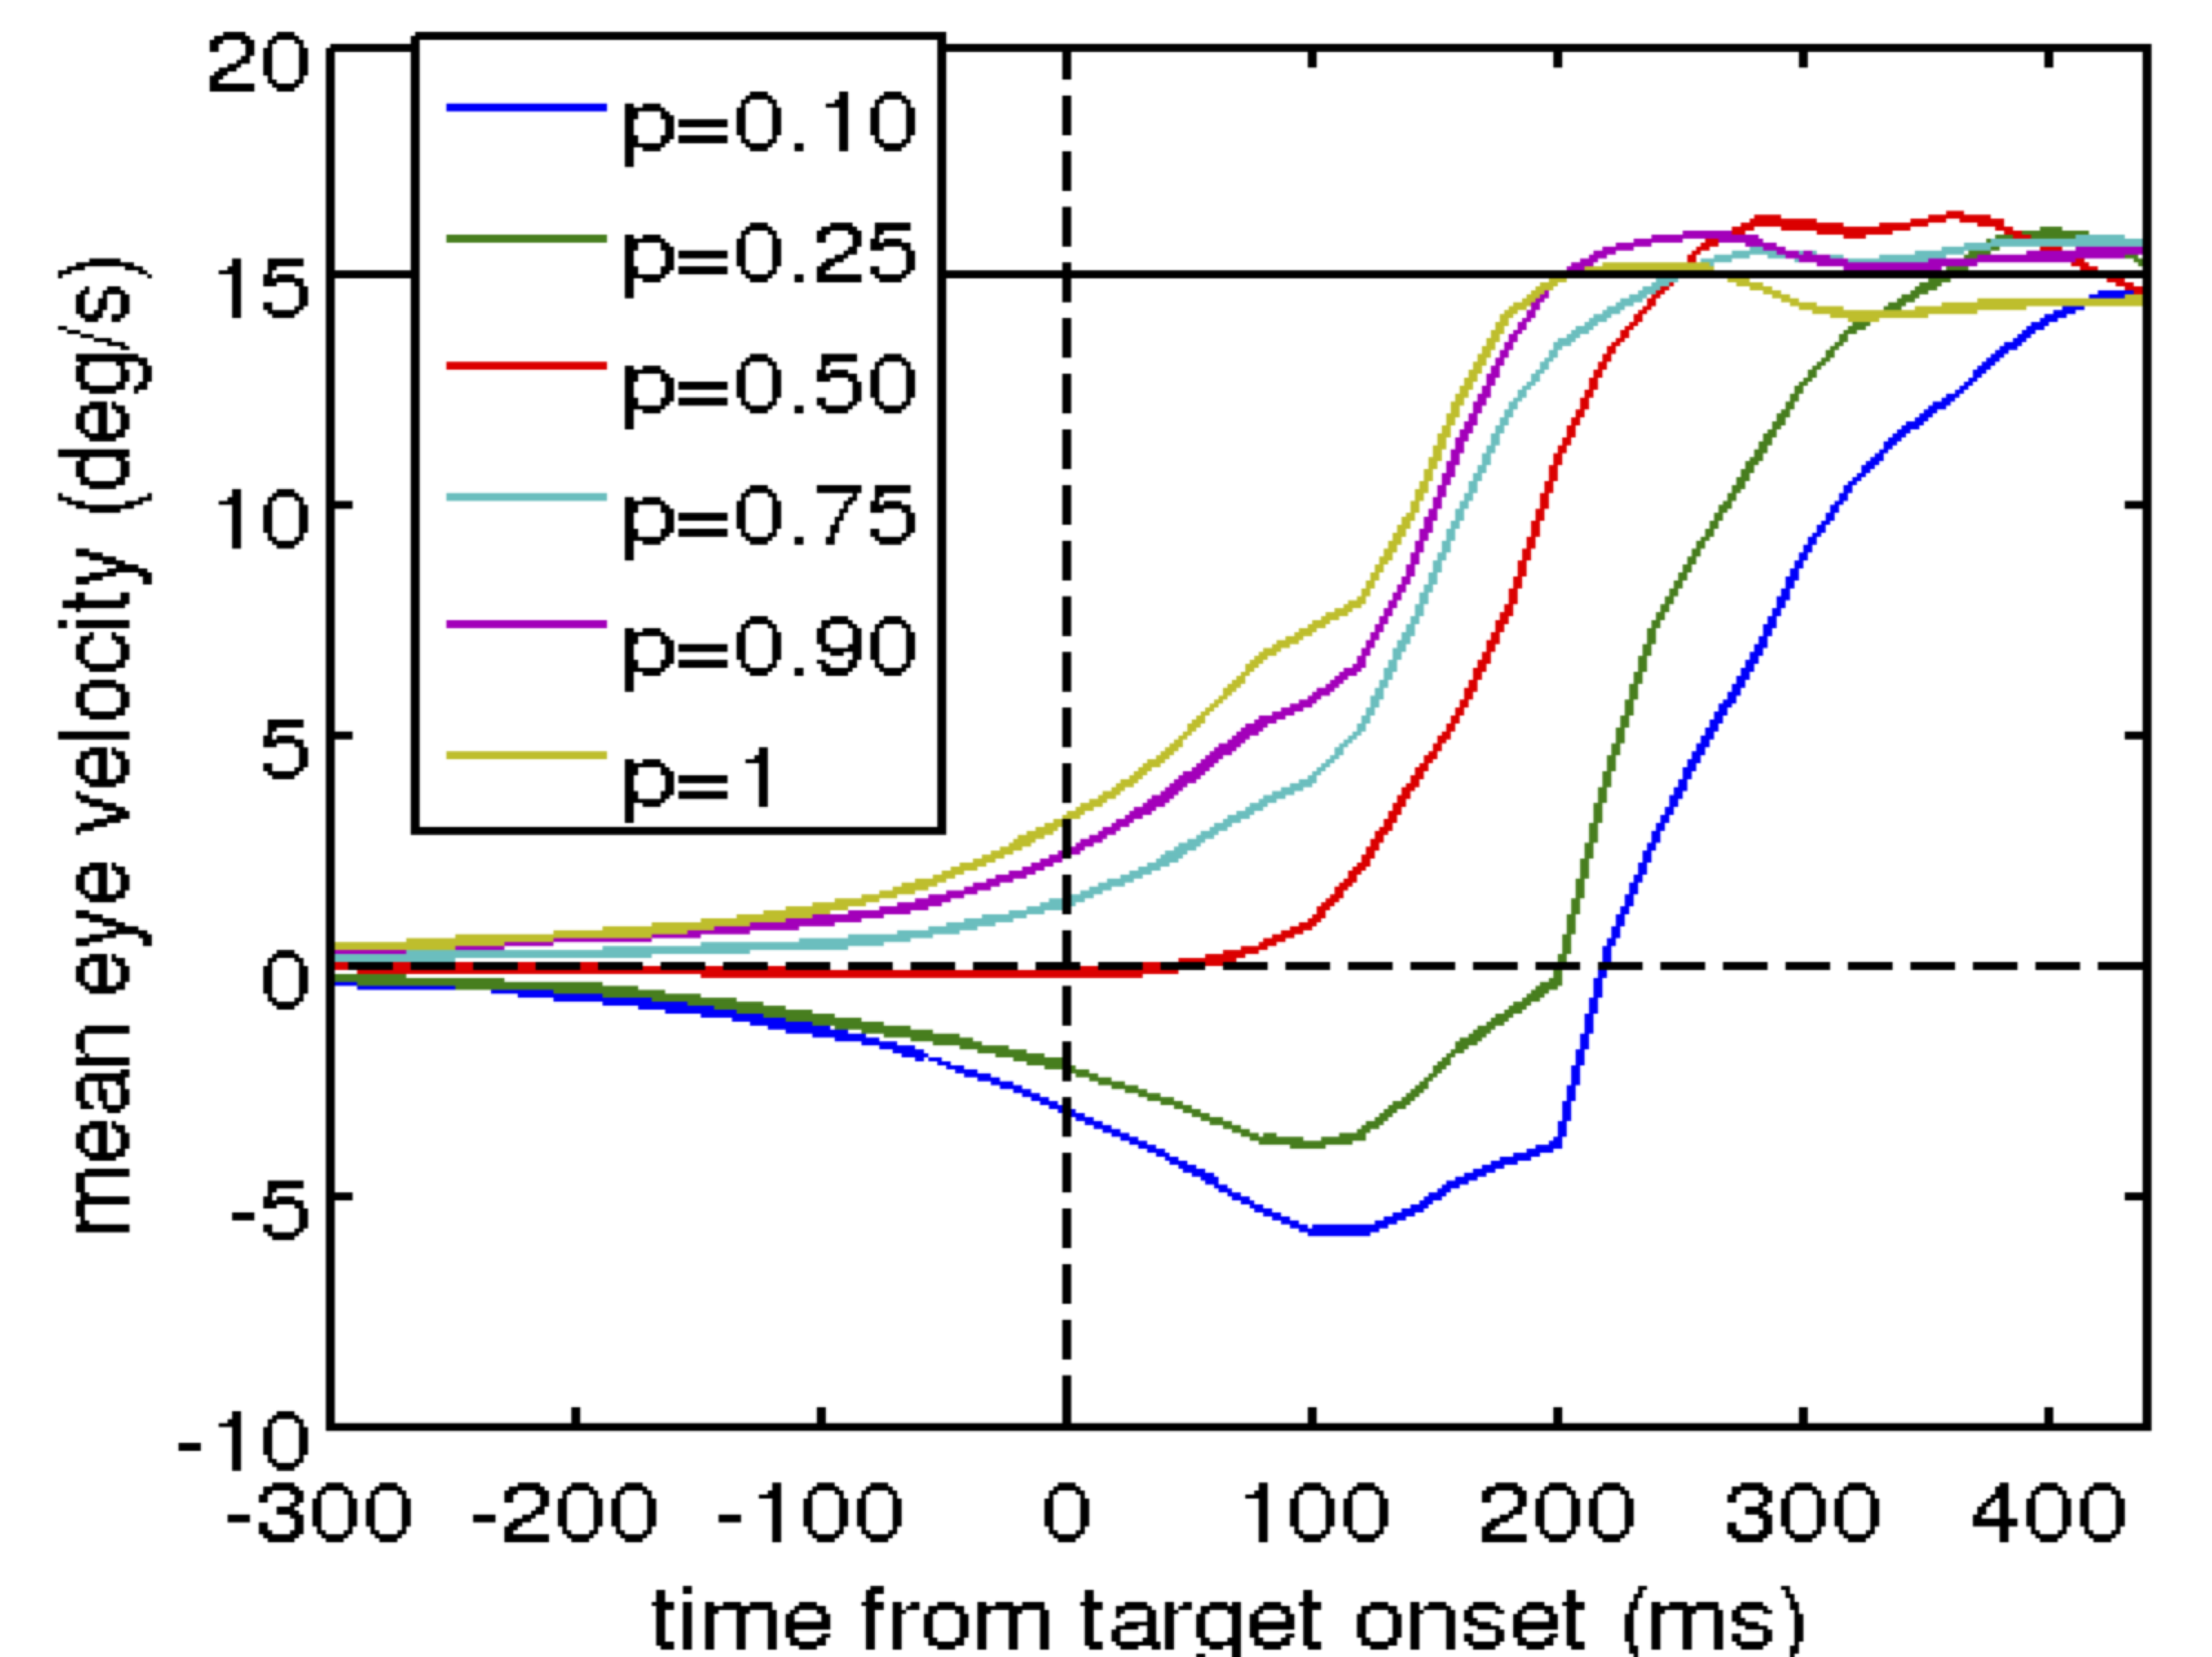
\includegraphics[width=.49\linewidth]{image_anna_1} & 	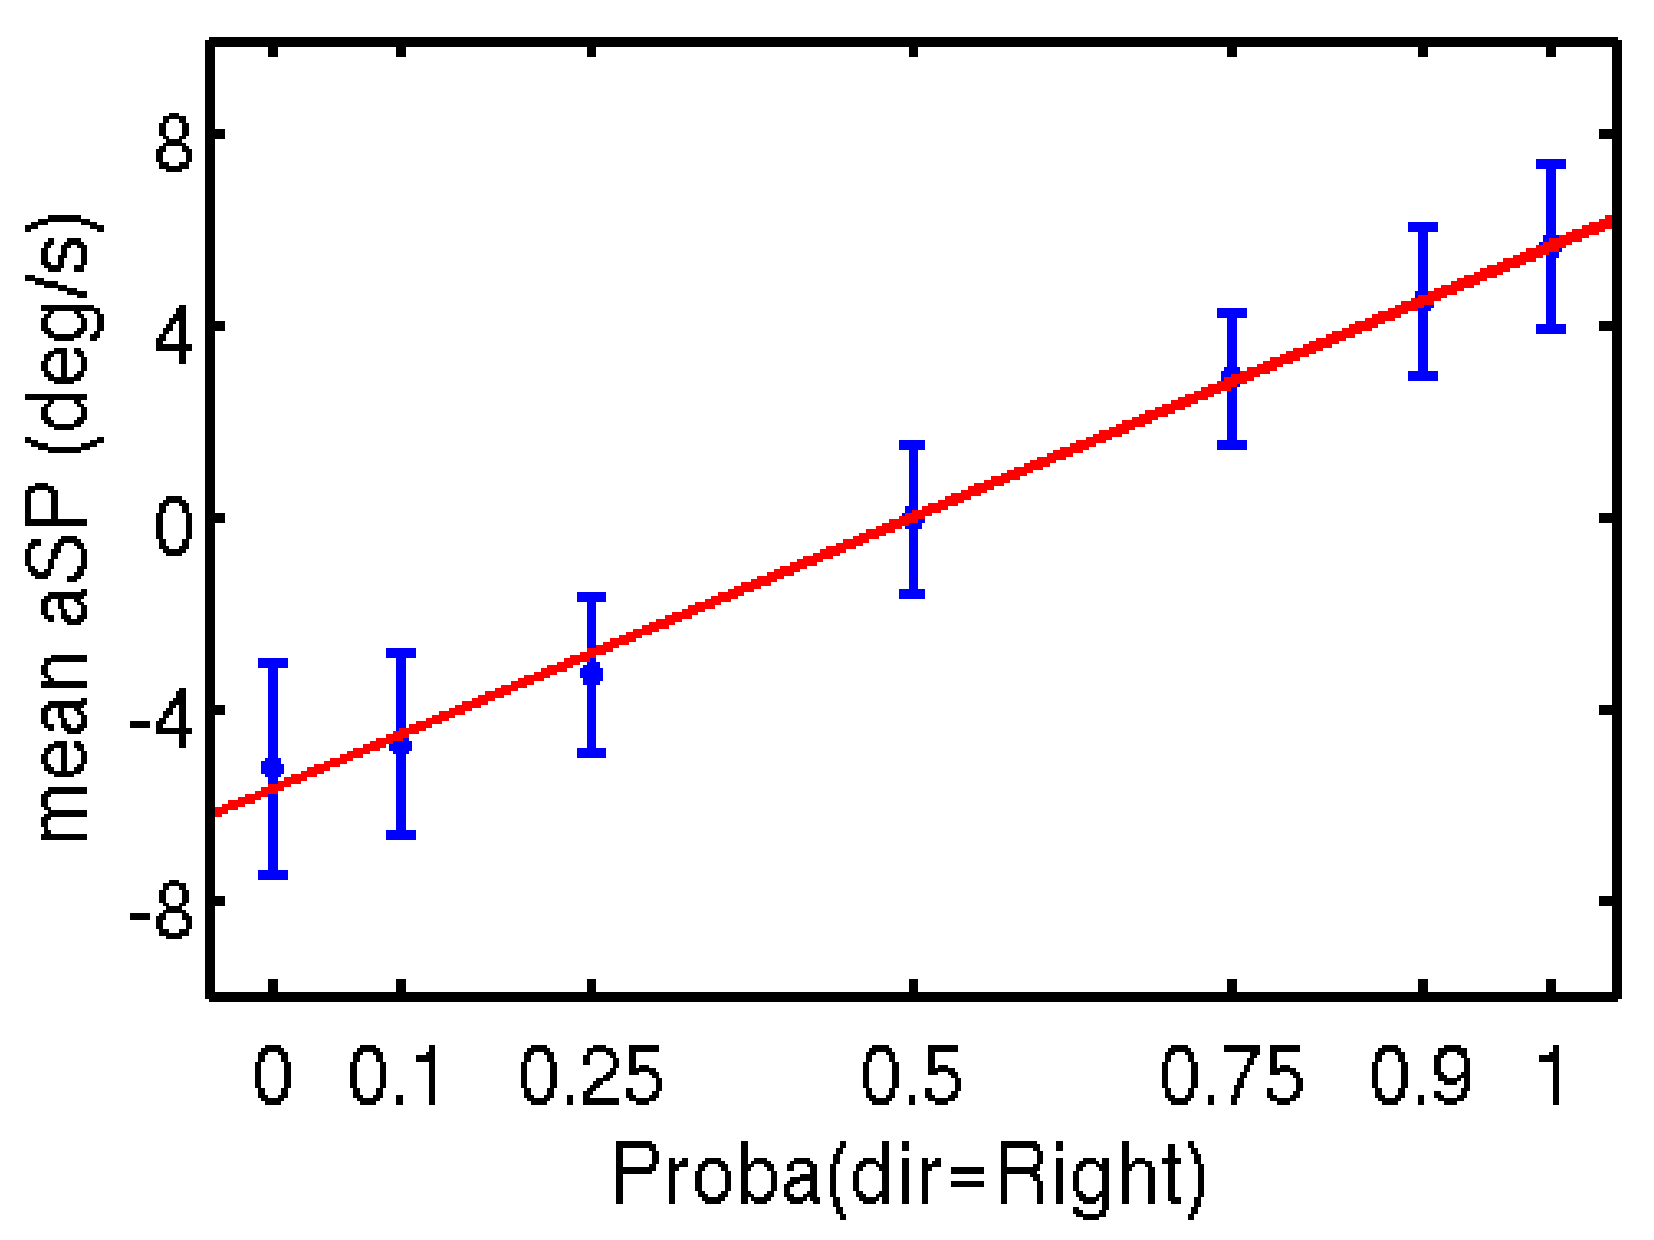
\includegraphics[width=.49\linewidth]{image_anna_2}
\end{tabular}
%\vspace{0.5cm}
%\begin{center}
%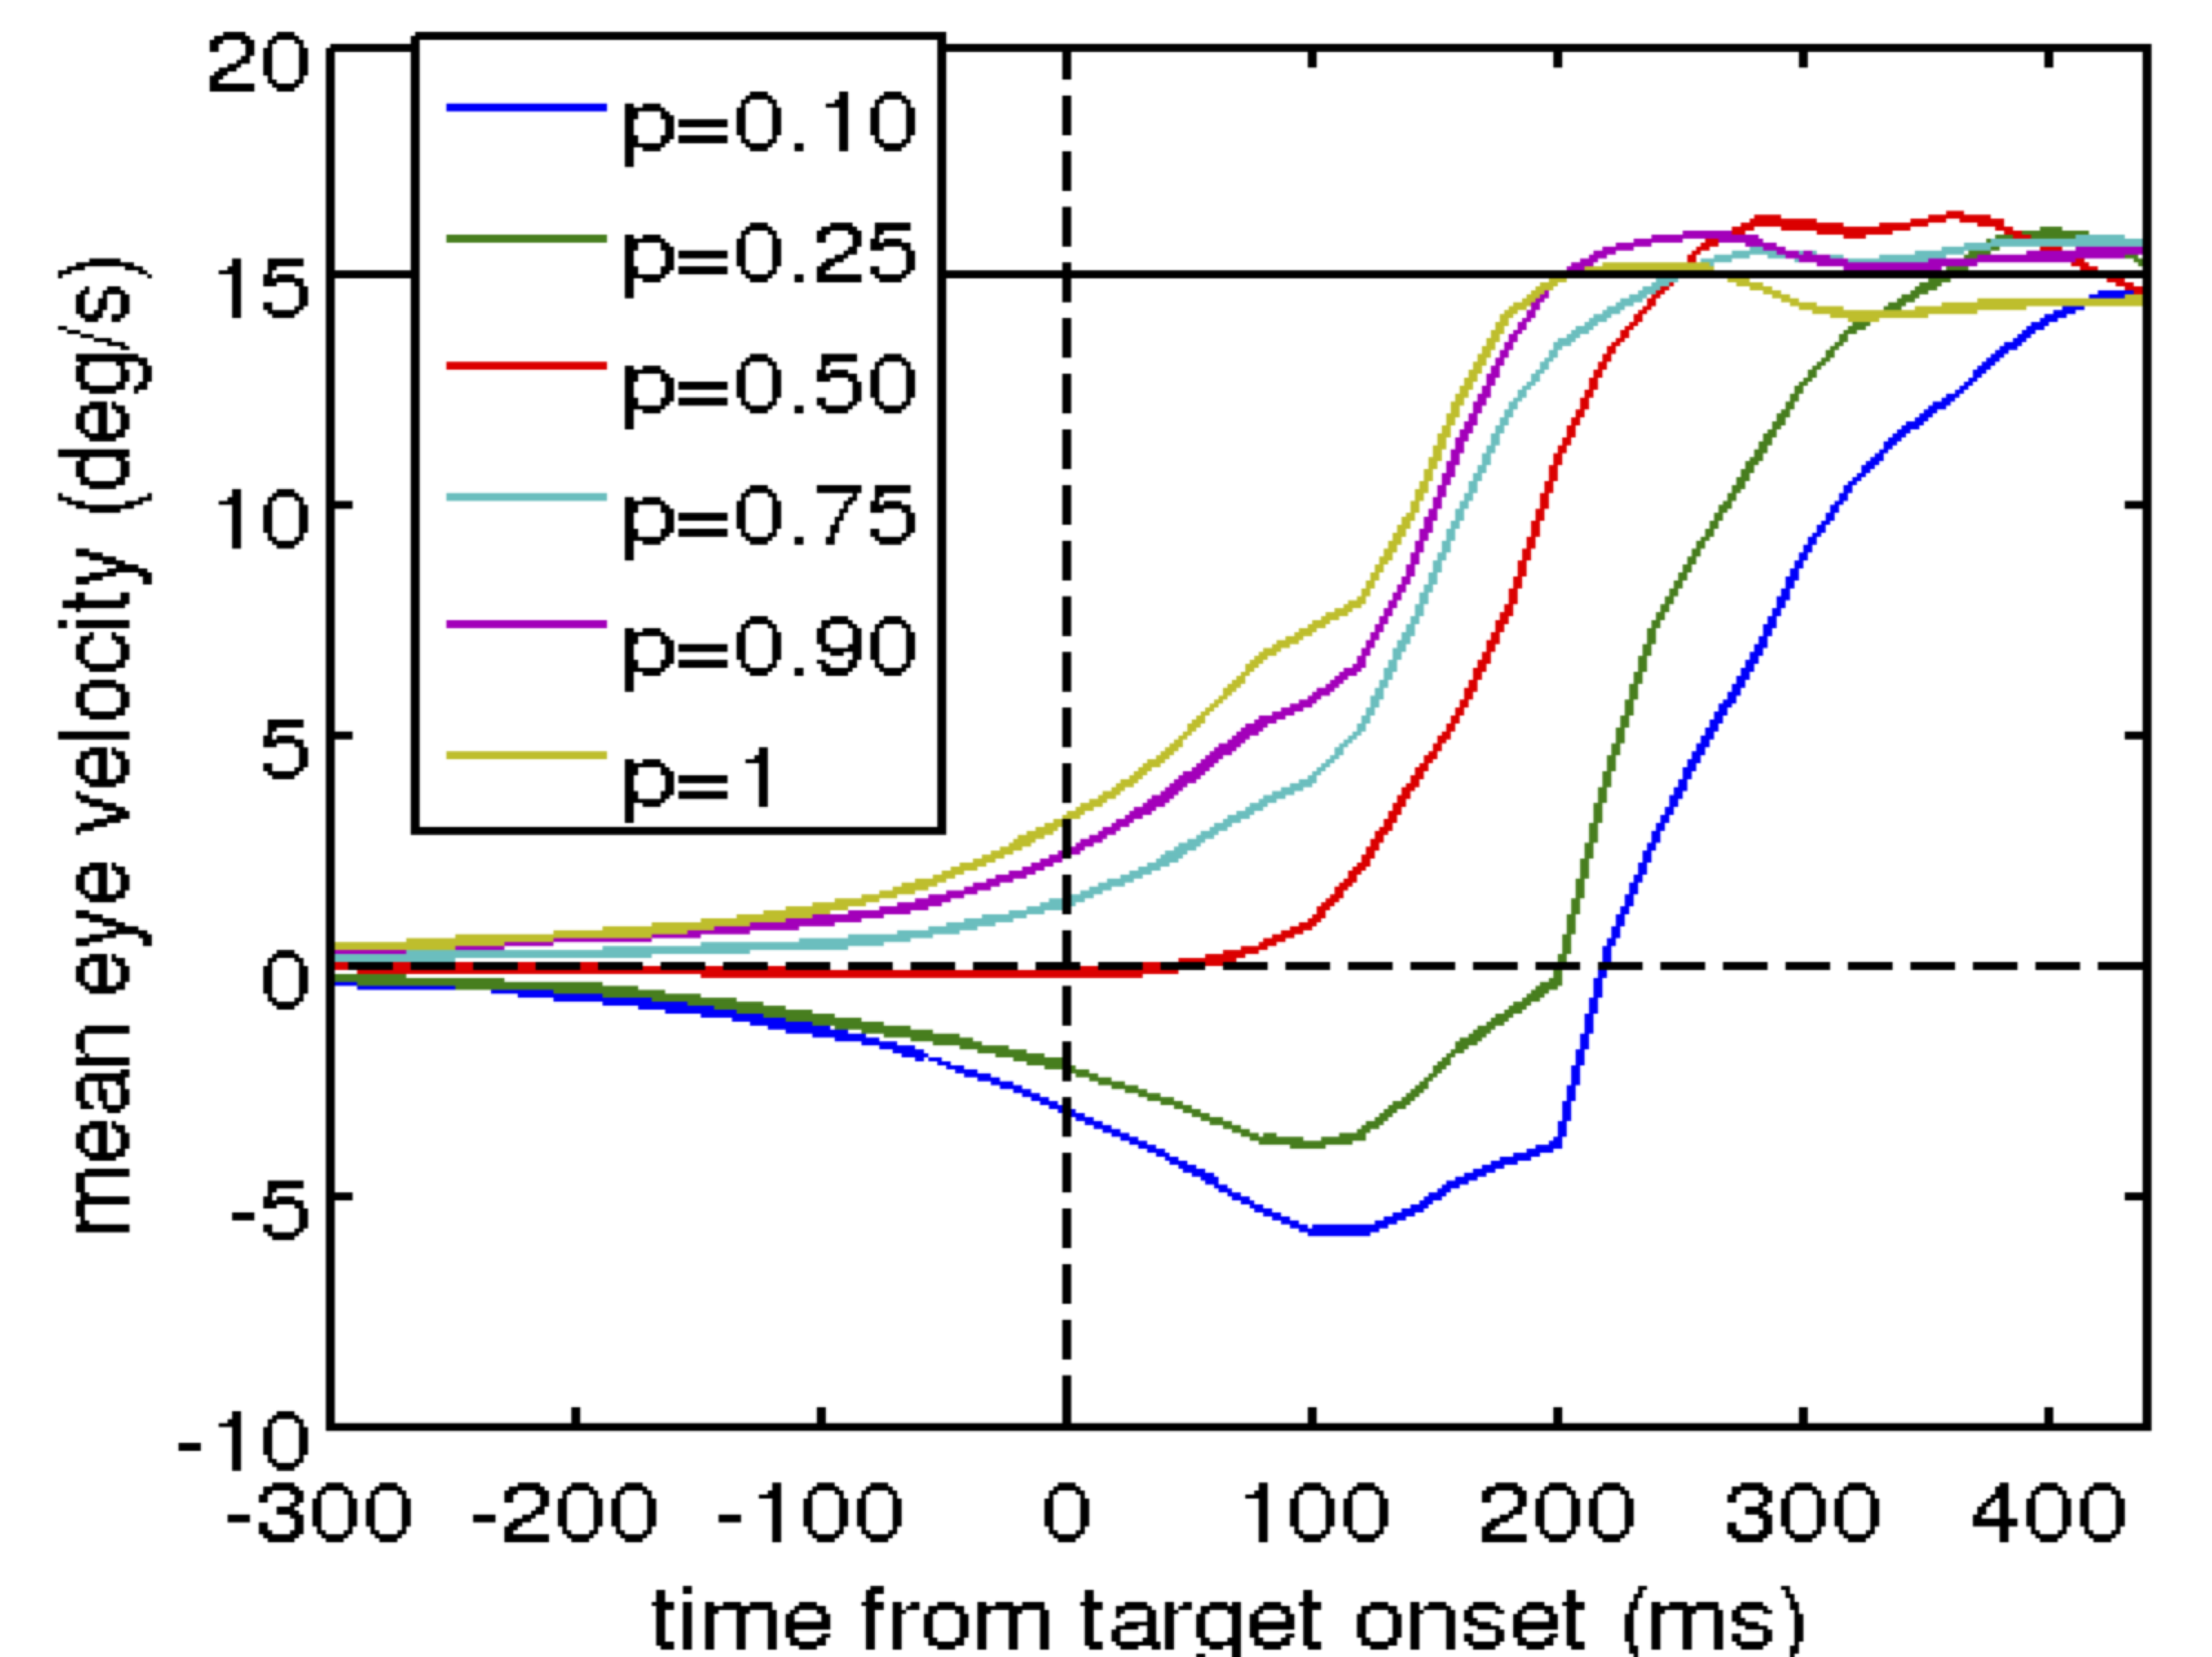
\includegraphics[width=0.9\linewidth]{image_anna_1}
%\end{center}
%\vspace{0.5cm}
%\begin{center}
%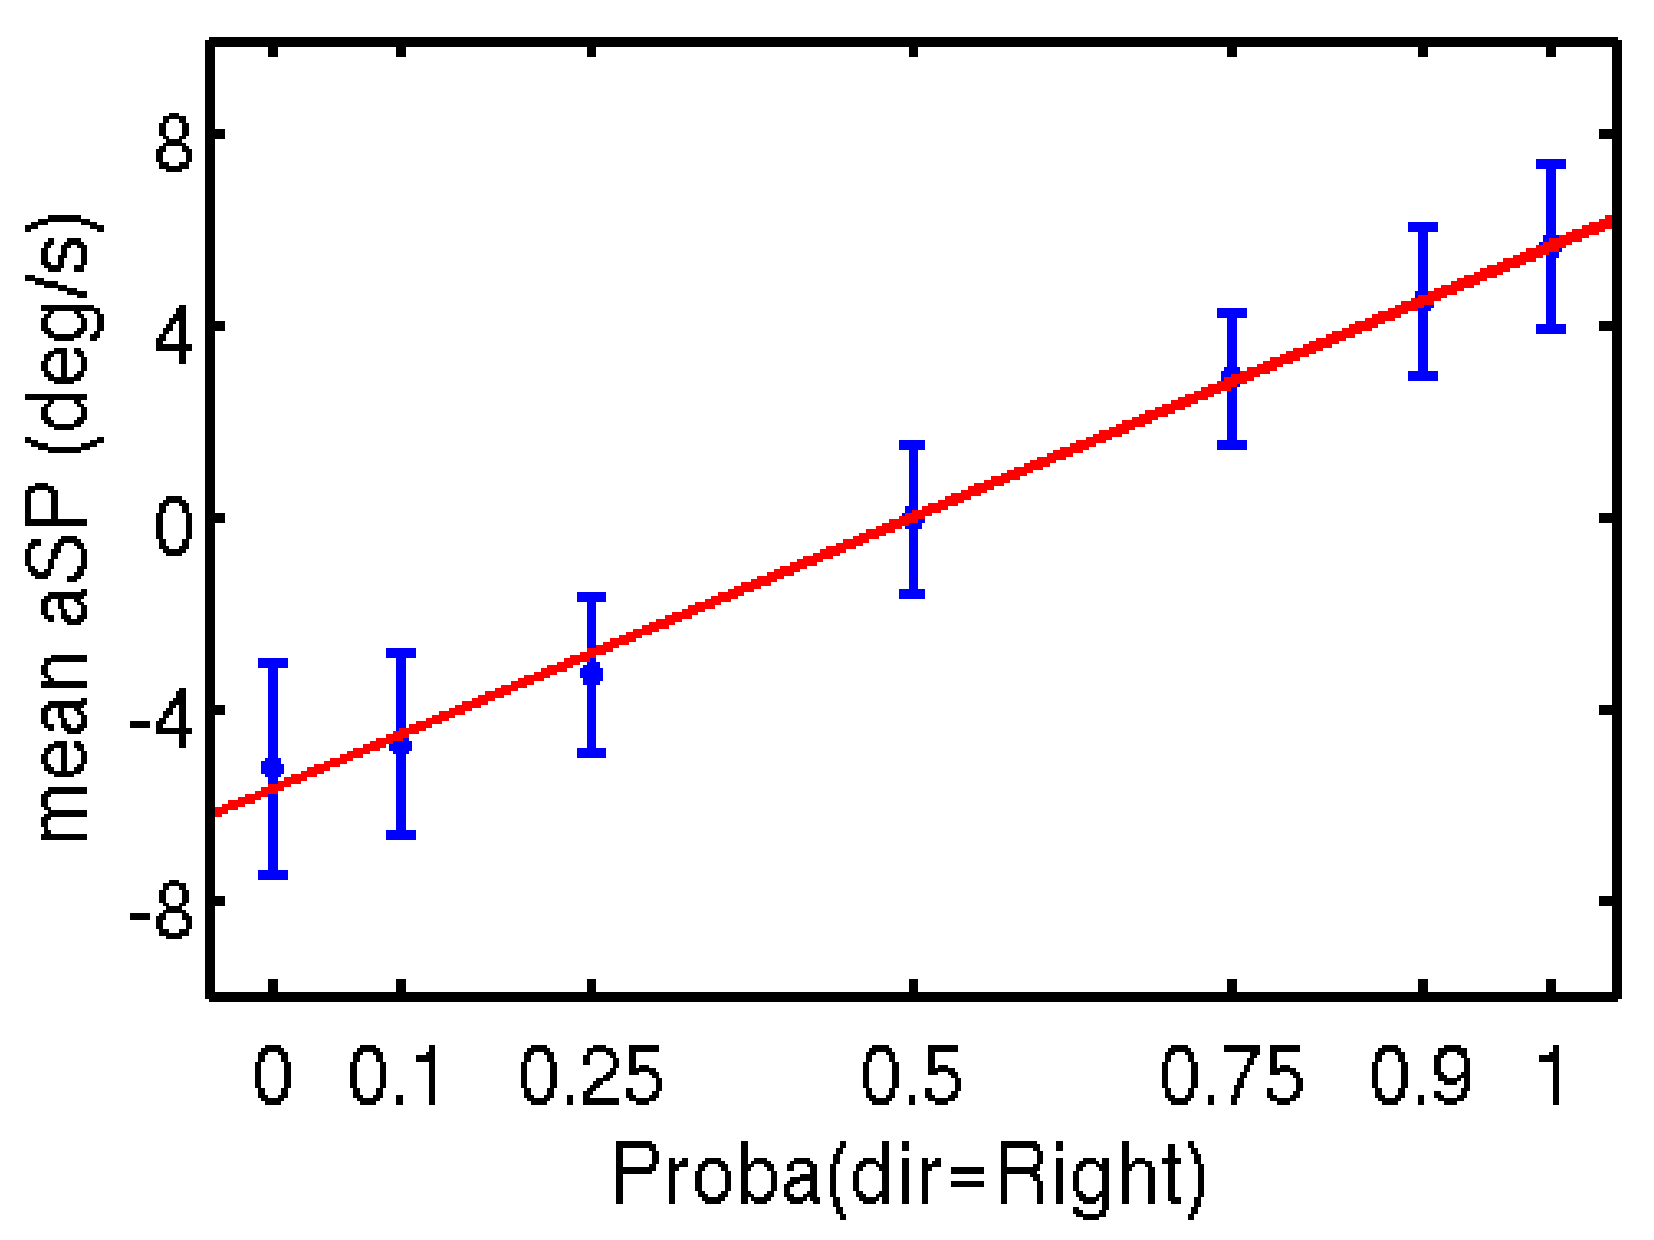
\includegraphics[width=0.9\linewidth]{image_anna_2}
%\end{center}
\caption{\emph{aSPEM} \textbf{(A)} 
\textbf{(B)} 
\textbf{(C)}  }
\label{fig:intro}
\end{figure}
%-------------------------------------------------------------%


However, such estimate may become particularly challenging in a dynamic context, where the probabilistic contingencies vary in time in an unpredictable way. In addition, whether and how the information processing underlying the buildup of aSPEM is linked to an explicit estimate of probabilities is unknown.


\section{Material and Method}

\subsection{Generative model: the switching model}

In order to answer these questions, we have set up an experiment comprising $3$ blocks of $200$ trials, see Figure~\ref{fig:protocole}-A\footnote{Each block is divided in 4 sub-blocks of $50$ trials as denoted by vertical black bars}. For each trial, a target makes either to the left or to the right, this direction being drawn from a Bernoulli process. The probability of this process varied in a piecewise-constant (that is, a step function varying between~$0$ and~$1$), similarly to~\textcite{Meyniel13}. The occurrence of these switches is itself drawn from a Bernoulli process of probability $p_{switch}=1/40$.

\eql{\choice{
x_0^t \eqdef o_t \propto \Bb(p^t) \\
x_1^t \eqdef p_t = p_{t-1} \quad \text{if} \quad s_t=0 \quad \text{and else} \quad p_t \propto \Jj \\
x_2^t \eqdef s_t \propto \Bb(\lambda) 
}}

where $\Jj = BB(\frac 1 2 , \frac 1 2 )$ is Jeffrey's prior
%-------------------------------------------------------------%
%: fig:protocole
\begin{figure}%[b!]
%\vspace{2mm}
\begin{center}
\textbf{(A)}     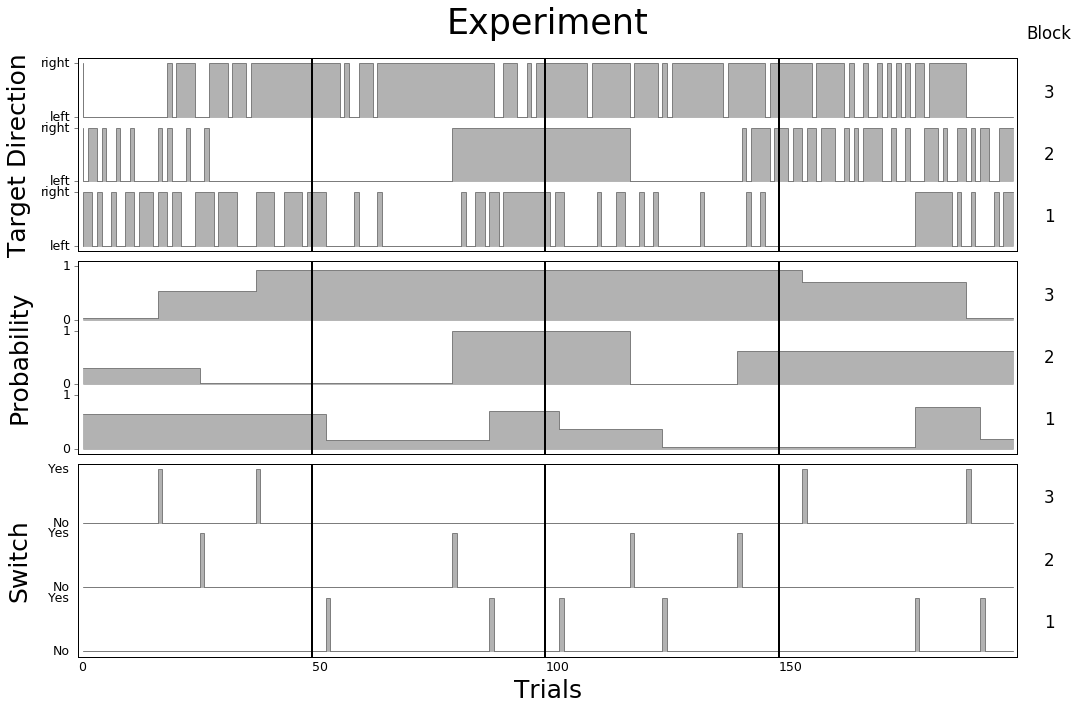
\includegraphics[width=.9\linewidth]{exp}
\textbf{(B)}     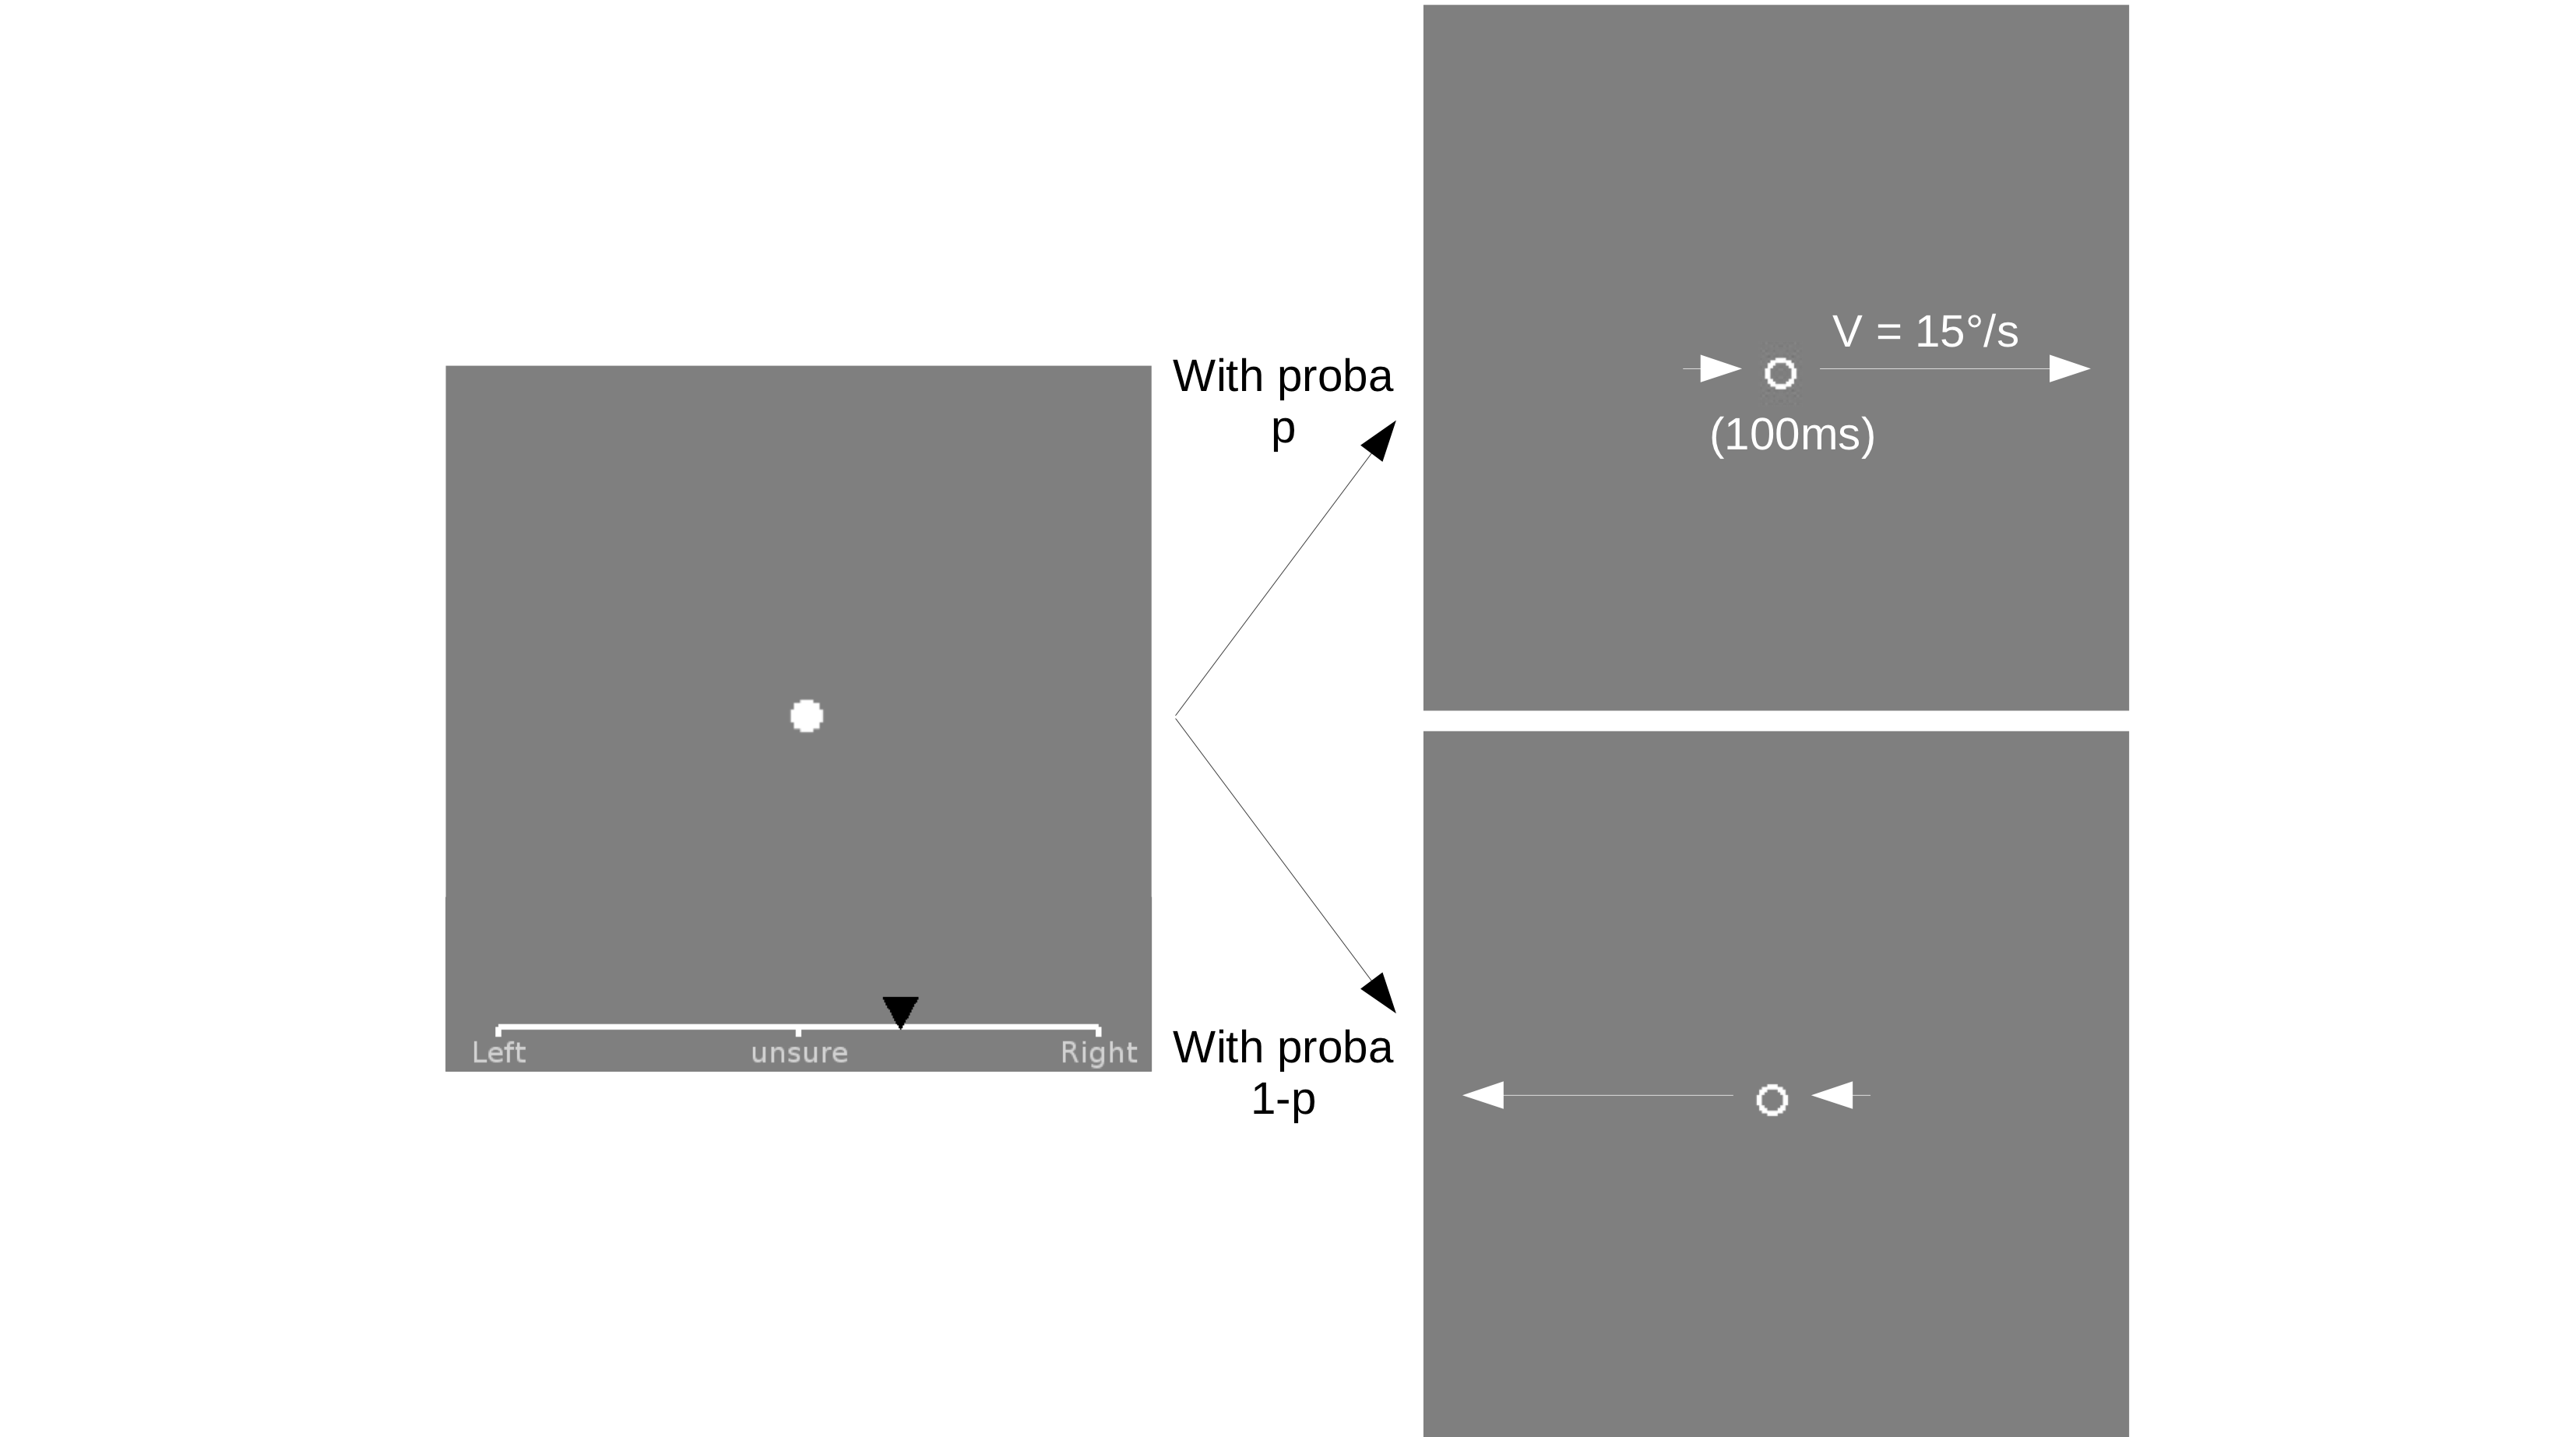
\includegraphics[width=.4\linewidth]{materiel_bet}
\textbf{(C)}     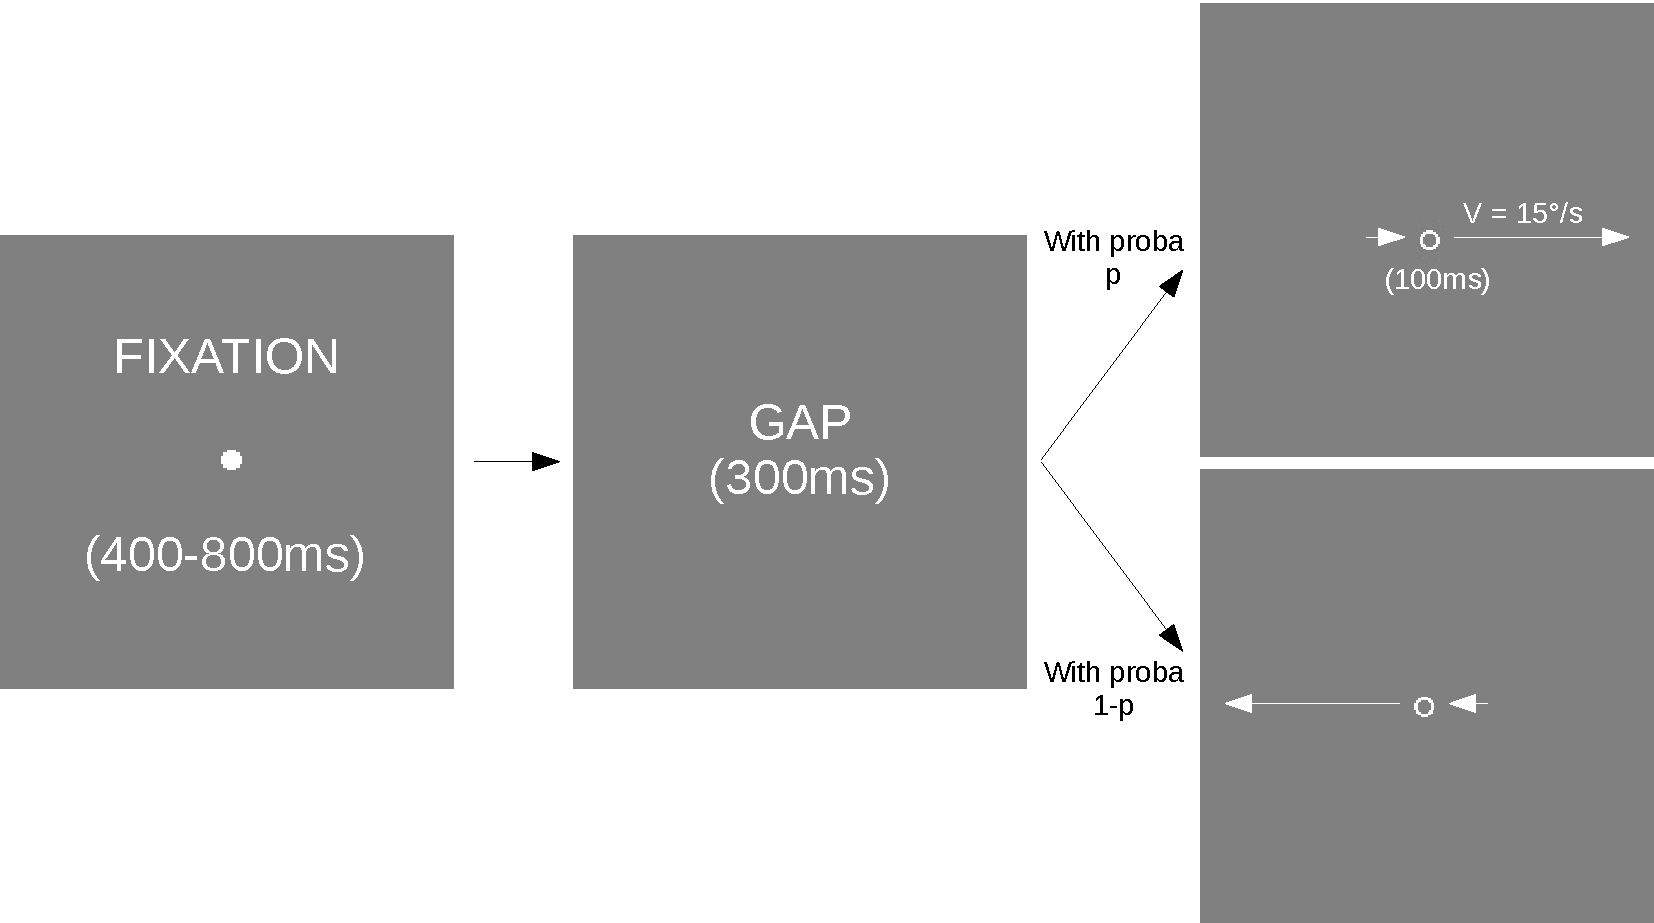
\includegraphics[width=.4\linewidth]{materiel_recording}
\end{center}
\caption{\emph{Protocol and previous results} \textbf{(A)} 
\textbf{(B)} 
\textbf{(C)}  }
\label{fig:protocole}
\end{figure}
%-------------------------------------------------------------%

We asked subjects to perform two tasks on different days :
%\begin{itemize}\setlength{\itemsep}{0ex}
%\item a <<Bet>>
%\item a <<recording>>
%\end{itemize}

\subsection{The Bet}
In this first part, the subjects must simply answer before each trial at the question \textit{ ``How sure are you that the target will go left or right''}. This was performed by adjusting a cursor on the screen using the mouse (see Figure).

%\subsection{The Bet}
%Example of results obtained during the bet :
%\begin{center} 
%    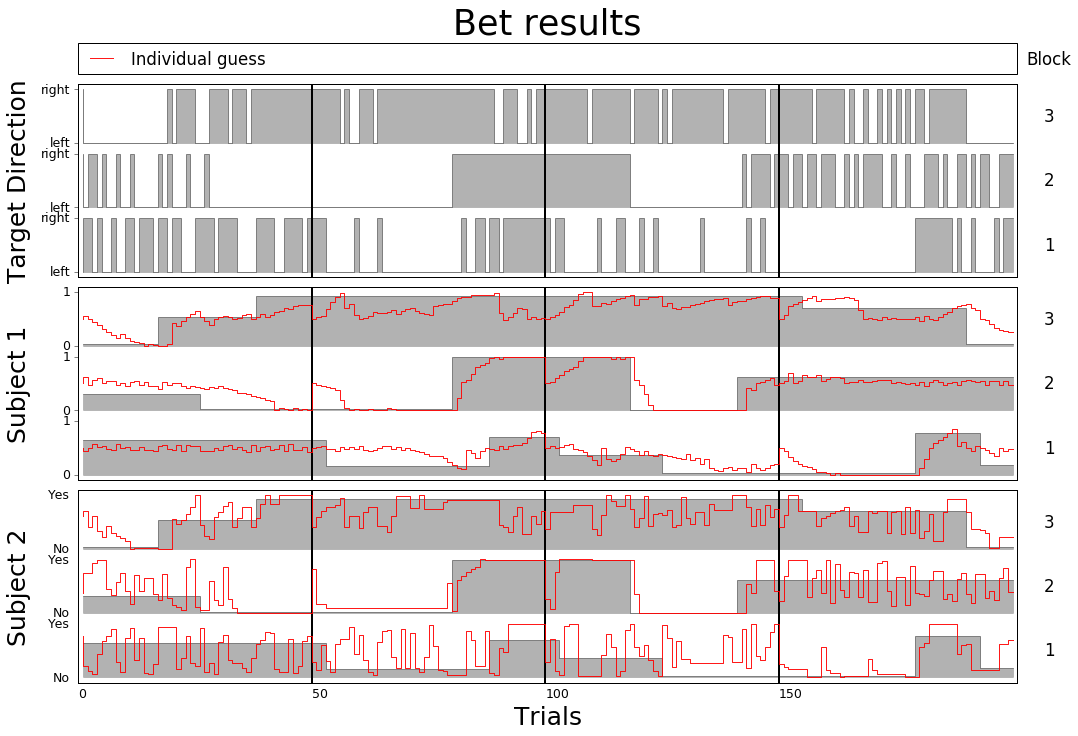
\includegraphics[width=1\linewidth]{results_pari}
%\end{center}
%%Comparison of probabilities bet with respect to the real probability :
%The scatter plot of the value of the bet (probability bet) as a function of the real probability at every given trial shows that there is a good correlation between both values:

%\begin{center}
%    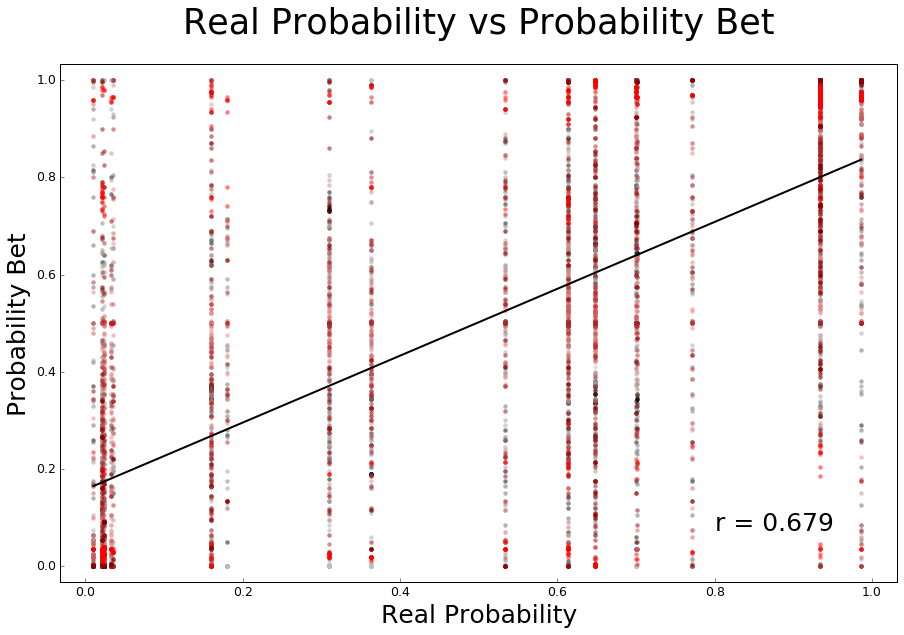
\includegraphics[width=1\linewidth]{p_real--p_bet}
%\end{center}

\subsection{Eye movements recording}
Then, we recorded their eye movements as they were tracking the target's motion. Importantly, we used that exact same sequence.

%
Stimuli were generated using Matlab 7.10.0 on a Mac running OS 10.6.8 and displayed on a 20" Viewsonic p227f monitor with resolution $1024\times 768$ at 100~\si{\Hz}. Psychophysics routines were written using Matlab and Psychtoolbox 3.0.9 controlled the stimulus display. Observers sat 57~\si{\cm} from the screen in a dark room. Six male observers with normal or corrected-to-normal vision took part in these experiments. They gave their informed consent and the experiments received ethical approval from the Aix-Marseille Ethics Committee in accordance with the declaration of Helsinki.


\subsection{Eye movements analysis}

In order to extract the relevant parameters of the oculomotor responses, we developed new tools based on a best-fitting procedure of predefined patterns and in particular the typical smooth pursuit velocity profile that was recorded for the aSPEM (Top row). This was applied to each trial individually, and we show below some prototypical example of respectively a neutral, anticipatory positive and anticipatory negative aSPEMs examples (respectively second to bottom rows) :

%-------------------------------------------------------------%
%: fig:eye_fits
\begin{figure}%[b!]
%\vspace{2mm}
\begin{center} 
    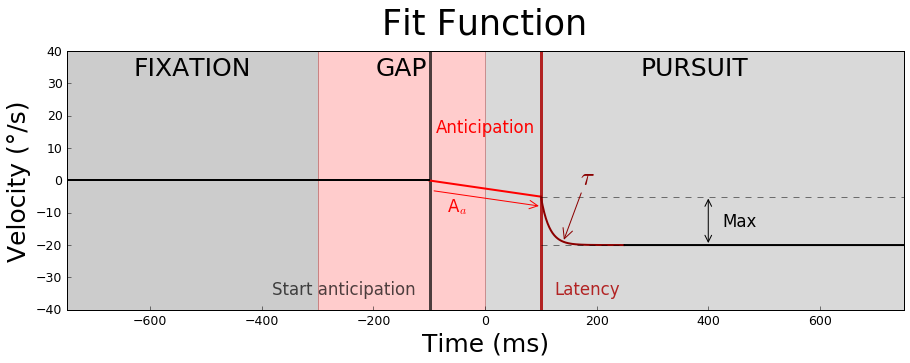
\includegraphics[width=1\linewidth]{Fonction_Fit}
    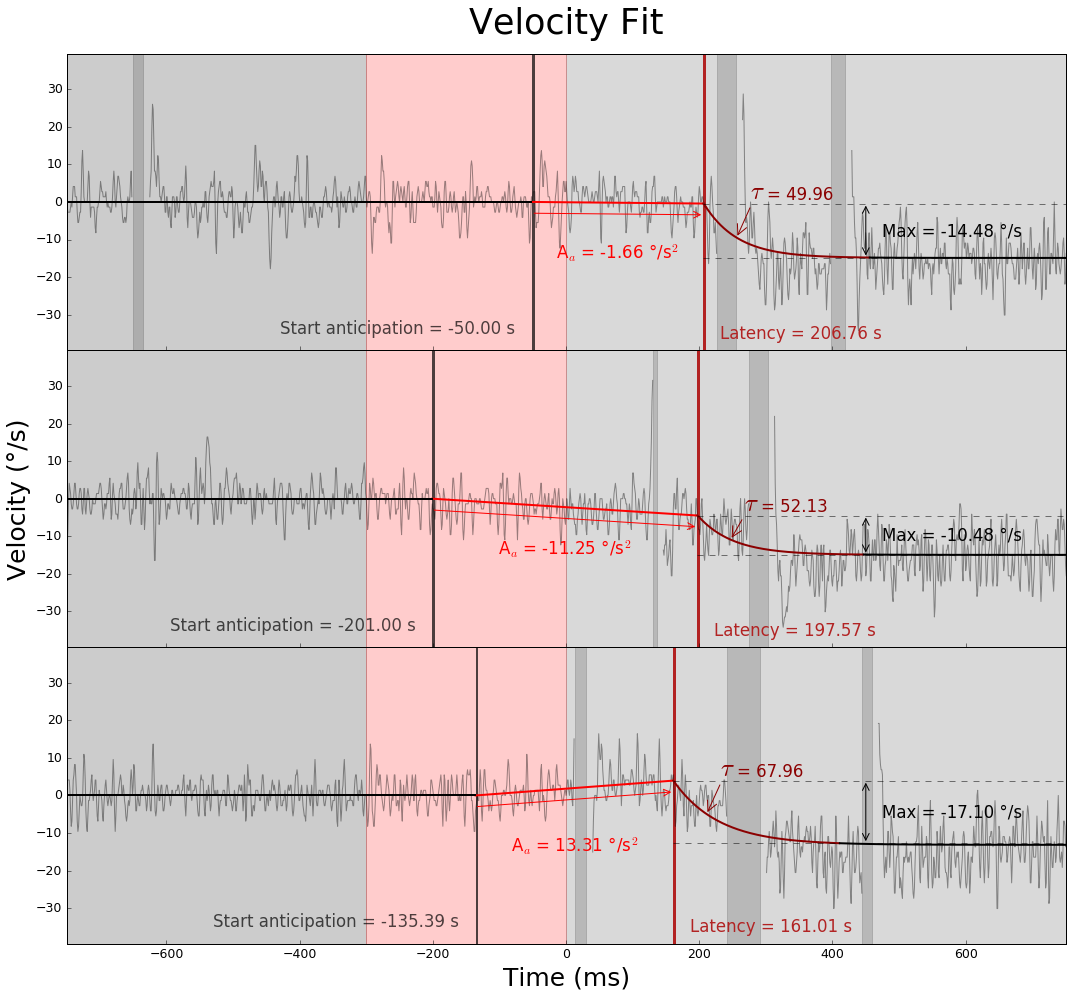
\includegraphics[width=1\linewidth]{Fit_vitesse}
\end{center}
\caption{\emph{Eye movements analysis} \textbf{(A)} 
\textbf{(B)} 
\textbf{(C)}  }
\label{fig:eye_fits}
\end{figure}
%-------------------------------------------------------------%


\section{Results: Bayesian change point model}

% https://github.com/laurentperrinet/bayesianchangepoint

\subsection{Bayesian change point model}

We have designed an agent adapted the Bayesian Online Change-point Detection model~\parencite{AdamsMackay2007}. This model uses a latent variable r which represents the length of the current interval during which motion-direction probability ($\hat{P}$) has not changed. The agent infers at each trial the likelihood  of r and then deduces the optimal $\hat{P}$ (we used the expected value and the max as readouts) and the uncertainty associated to it. We simulated the model across our experimental sequences, as illustrated by the example for the third block.

%-------------------------------------------------------------%
%: fig:results_bcp
\begin{figure}%[b!]
%\vspace{2mm}

\begin{center} 
    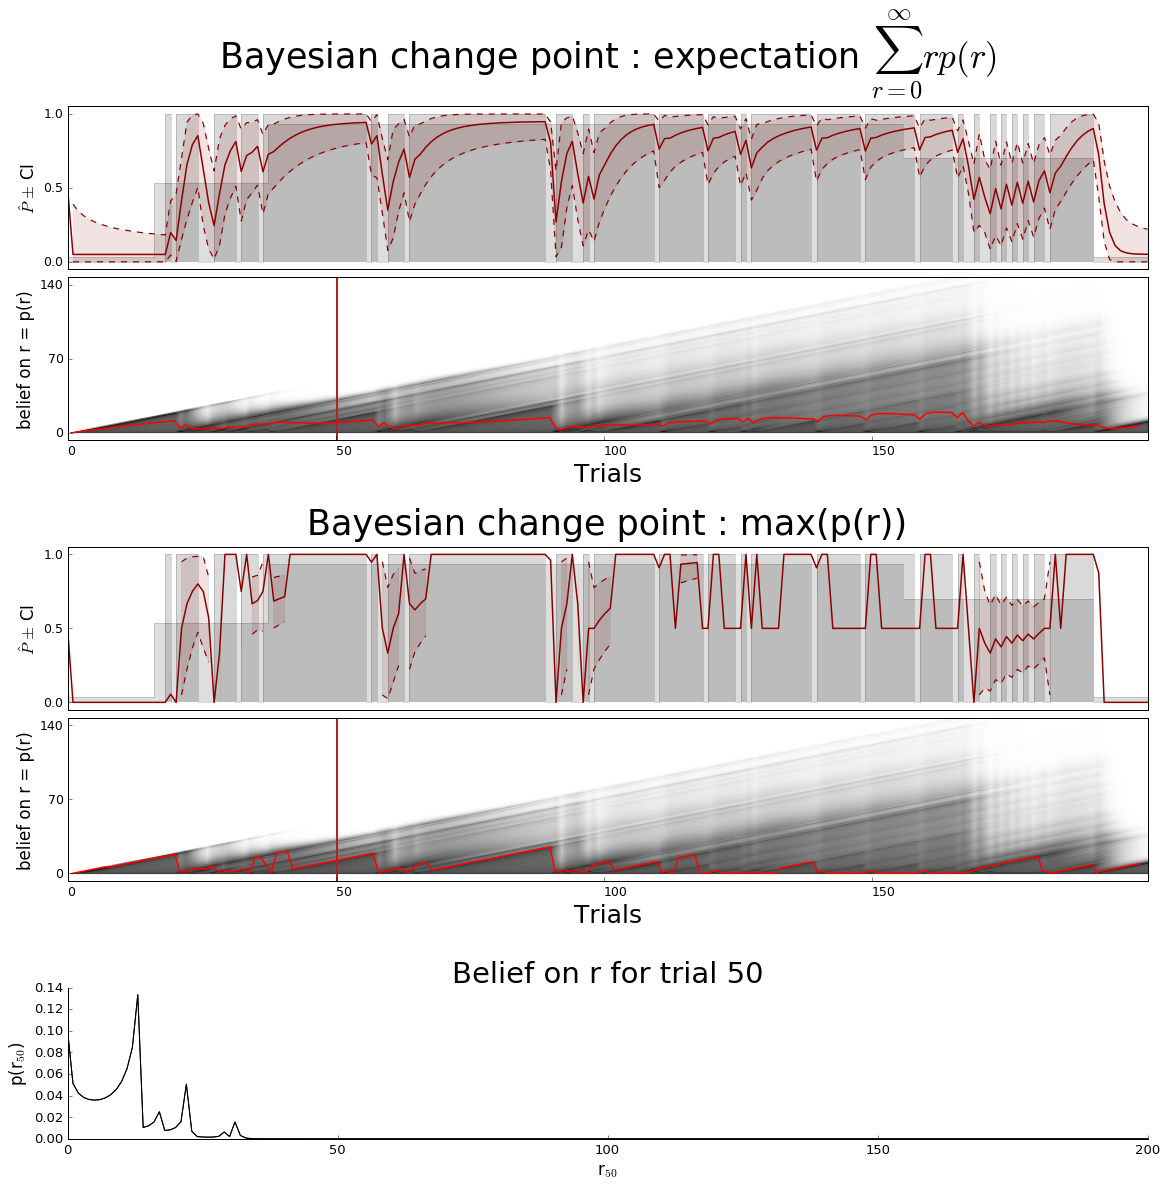
\includegraphics[width=1\linewidth]{bayesianchangepoint}
\end{center}

%\begin{center} 
%    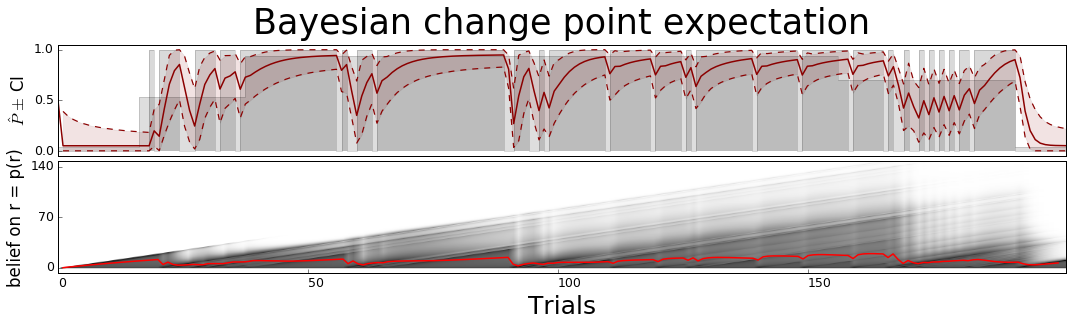
\includegraphics[width=1\linewidth]{bayesianchangepoint_e}
%\end{center}

%\begin{center} 
%    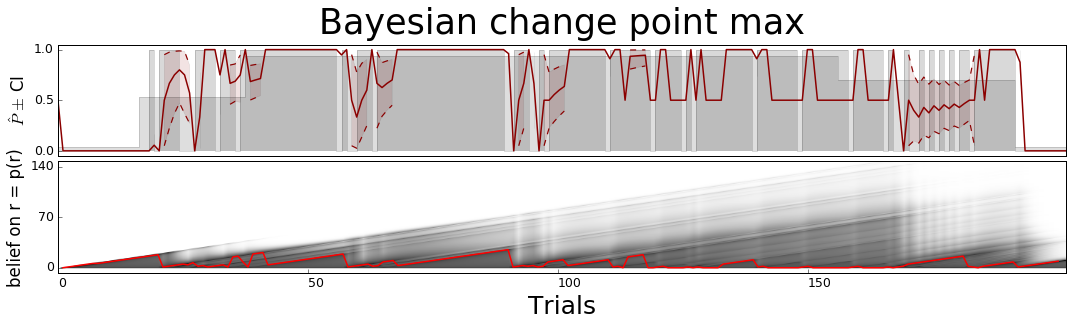
\includegraphics[width=1\linewidth]{bayesianchangepoint_m}
%\end{center}
\caption{\emph{Bayesian change point model} \textbf{(A)} 
\textbf{(B)} 
\textbf{(C)}  }
\label{fig:results_bcp}
\end{figure}
%-------------------------------------------------------------%




Computing the likelihood:
The main difference between our algorithm and that of Wilson is the way that the likelihood is computed.

\subsection{Bayesian change point algorithm}

To summarize, the algorithm 

\begin{enumerate}
	\item     Initialize

	\begin{itemize}
		\item    $P(r_0)= S(r)$ or $P(r_0=0)=1$ and
		\item    $\nu^{(0)}1 = \nu_{prior}$ and $\chi^{(0)}1 = \chi_{prior}$
	\end{itemize}

	\item    Observe New Datum $x_t$
    \item    Evaluate Predictive Probability $\pi_{1:t} = P(x |\nu^{(r)}_t,\chi^{(r)}_t)$
    \item    Calculate Growth Probabilities $P(r_t=r_{t-1}+1, x_{1:t}) = P(r_{t-1}, x_{1:t-1}) \pi^{(r)}_t (1-H(r^{(r)}_{t-1}))$
    \item    Calculate Changepoint Probabilities $P(r_t=0, x_{1:t})= \sum_{r_{t-1}} P(r_{t-1}, x_{1:t-1}) \pi^{(r)}_t \cdot H(r^{(r)}_{t-1})$
    \item    Calculate Evidence $P(x_{1:t}) = \sum_{r_{t-1}} P (r_t, x_{1:t})$
    \item    Determine Run Length Distribution $P (r_t | x_{1:t}) = P (r_t, x_{1:t})/P (x_{1:t}) $
    \item    Update Sufficient Statistics :
	\begin{itemize}
		\item    $\nu^{(0)}_{t+1} = \nu_{prior}$, $\chi^{(0)}_{t+1} = \chi_{prior}$
		\item    $\nu^{(r+1)}_{t+1} = \nu^{(r)}_{t} +1$, $\chi^{(r+1)}_{t+1} = \chi^{(r)}_{t} + u(x_t)$
	\end{itemize}

    \item    Perform Prediction $P (x_{t+1} | x_{1:t}) = P (x_{t+1}|x_{1:t} , r_t) P (r_t|x_{1:t})$
    \item    go to (2)
\end{enumerate}


where $\KL{\hat p}{p}$ is the Kullback-Leibler divergence between samples $\hat p$ and model $p$ under a Bernouilli distribution
\begin{equation}
\KL{\hat p}{p} = \hat{p} \log\pa{\frac{\hat p}{p}} + (1-\hat p) \log\pa{\frac{1-\hat p}{1-p}}.
\end{equation}




\section{Results}


\subsection{Eye movements recording and the Bet}
%Example of results obtained during the recording overlaid with the results of the bet experiment :

Example of results obtained during the bet and the recording :

%\begin{center}
%    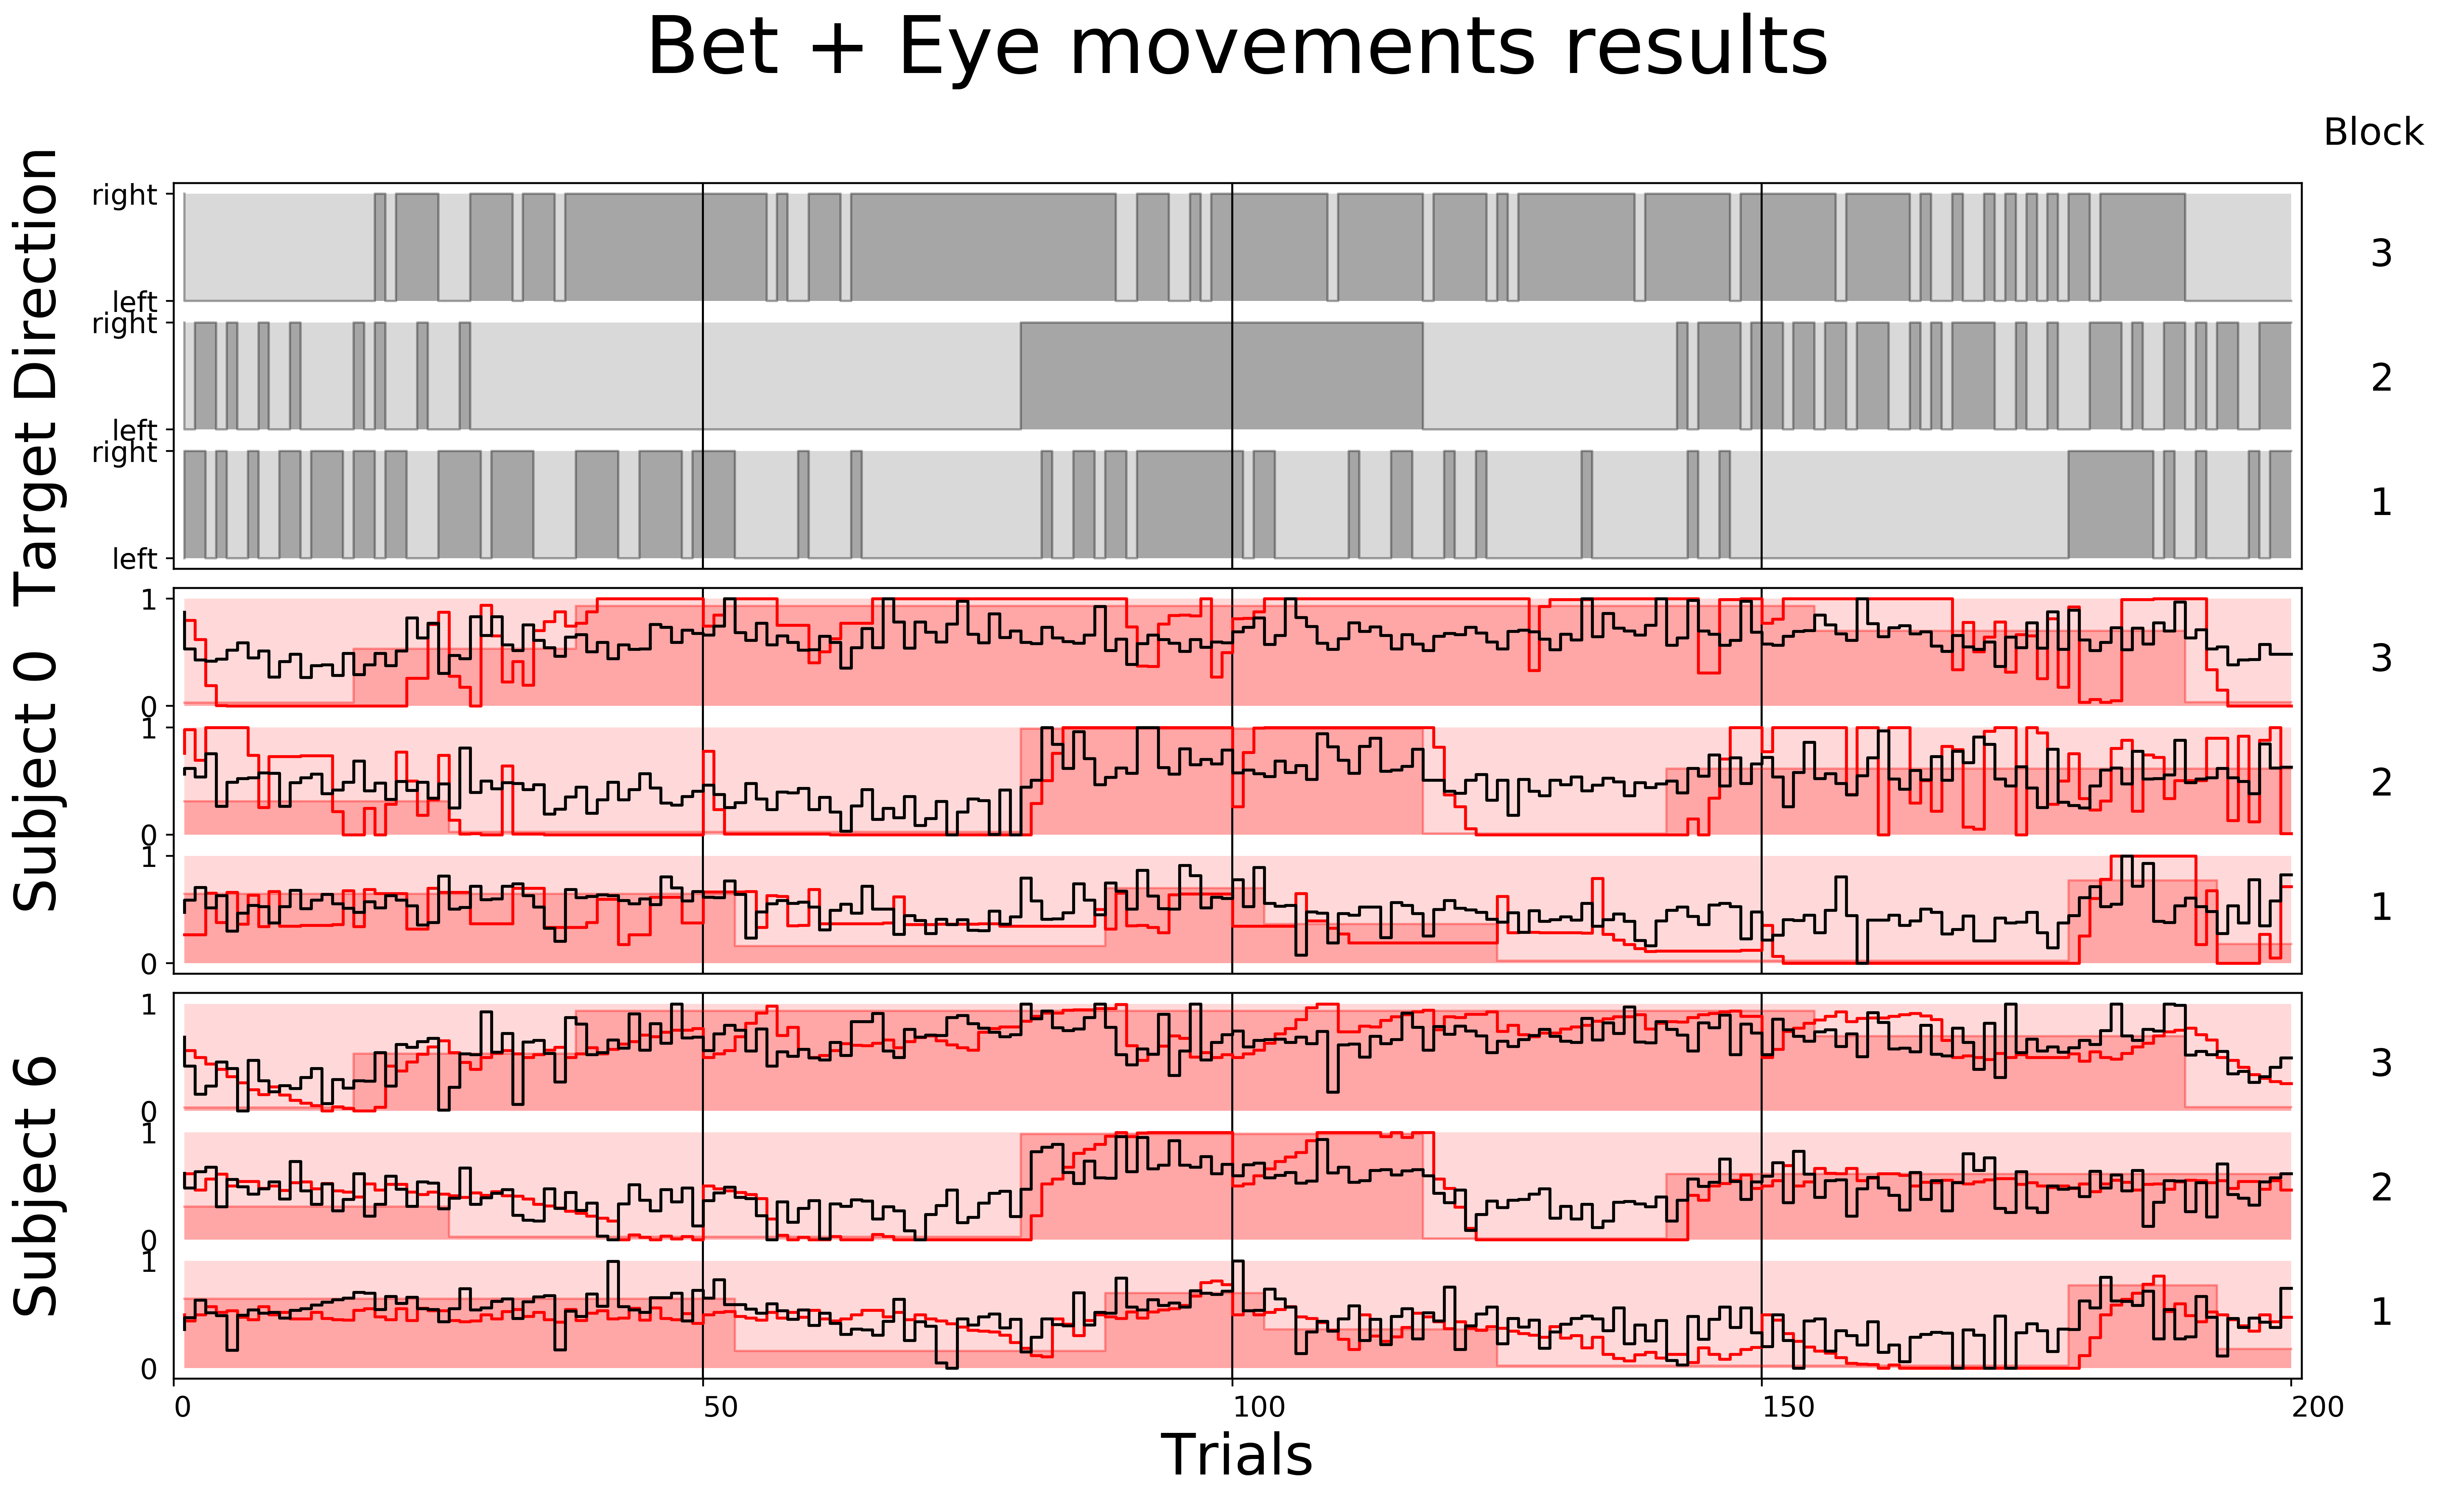
\includegraphics[width=1\linewidth]{results_enregistrement}
%\end{center}

%Let's plot the acceleration of anticipation (slope of aSPEM) as a function of the real probability at every given trial :

%\begin{center} 
%    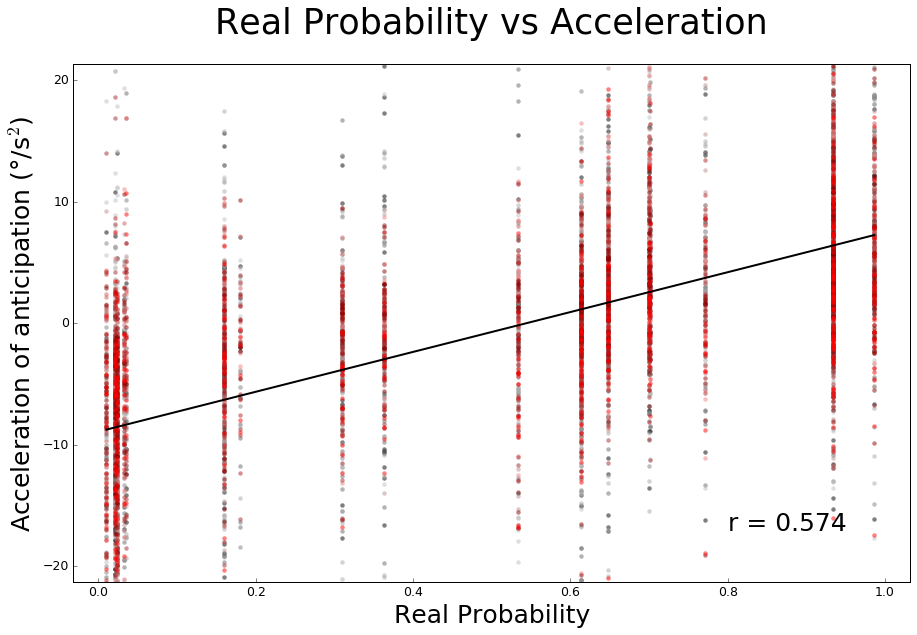
\includegraphics[width=1\linewidth]{p_real--v_a}
%\end{center}

Let's plot the value of the bet (probability bet)  and the acceleration of anticipation (slope of aSPEM) as a function of the real probability at every given trial :
%
%\begin{center} 
%    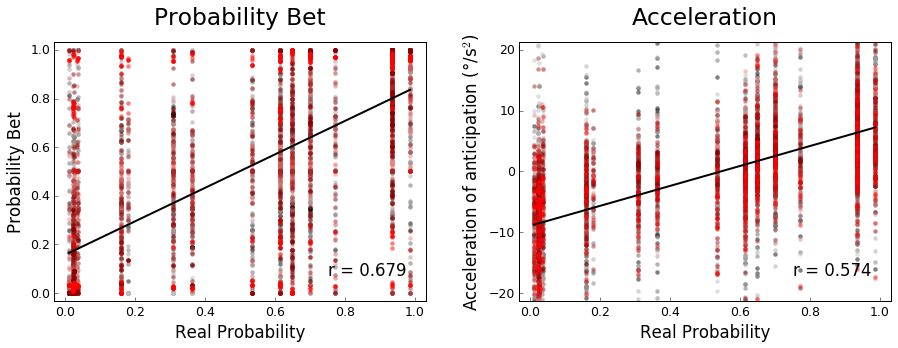
\includegraphics[width=1\linewidth]{P_real}
%\end{center}

Which give a strong and positive Pearson coefficient.

\subsection{Relating the Bet to the Recording}

We now compare the value of bet during the bet experiment with the acceleration of anticipation during the recording :

%\begin{center} 
%    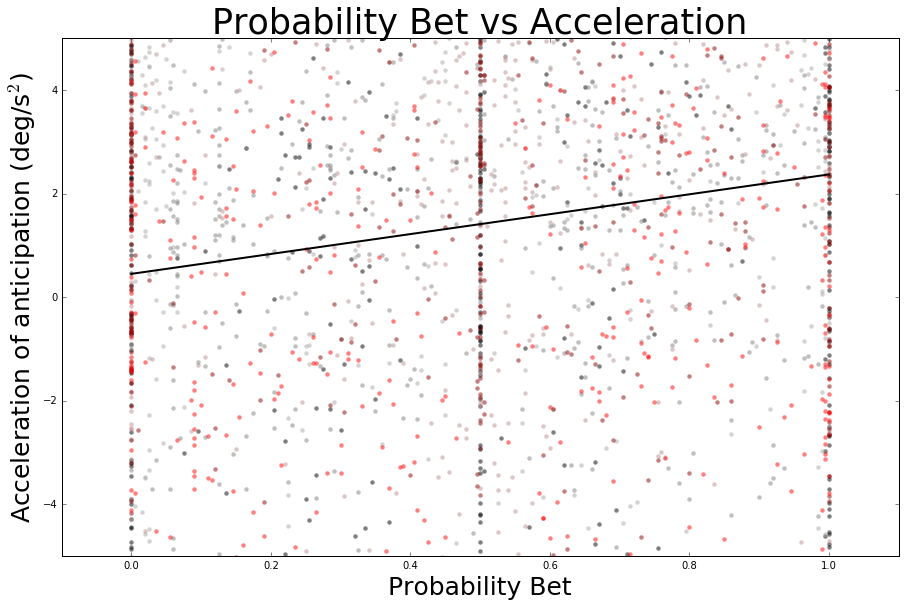
\includegraphics[width=1\linewidth]{p_parie--v_a}
%\end{center}

%\begin{center} 
%    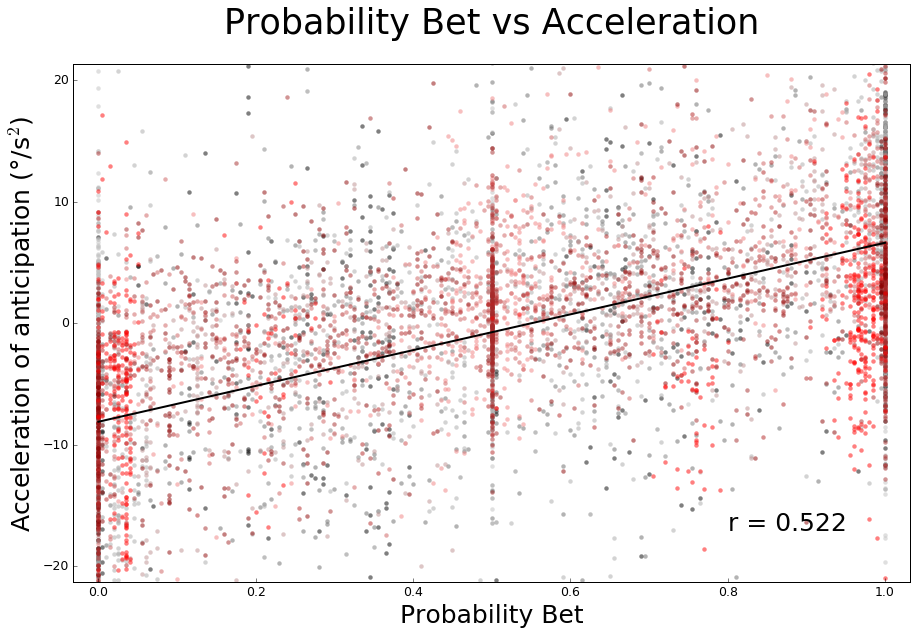
\includegraphics[width=1\linewidth]{p_bet--v_a}
%\end{center}

\subsection{Comparing the Bayesian change point model with humans}

We now compare the individual guesses during the bet experiment and the acceleration of anticipation during the eye movement recordings with the model simulations :


%-------------------------------------------------------------%
%: fig:results_psycho
\begin{figure}%[b!]
%\vspace{2mm}

\begin{center} 
    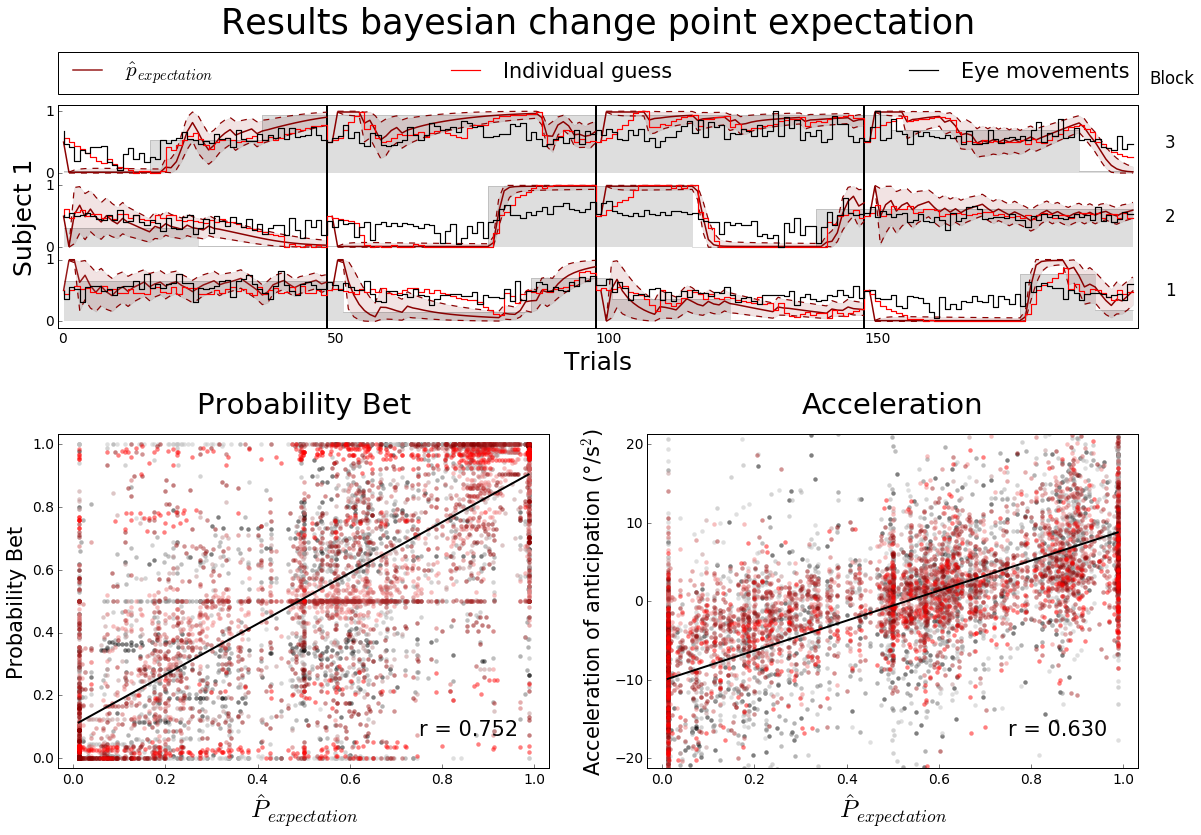
\includegraphics[width=1\linewidth]{results_bayesianchangepoint_e}
    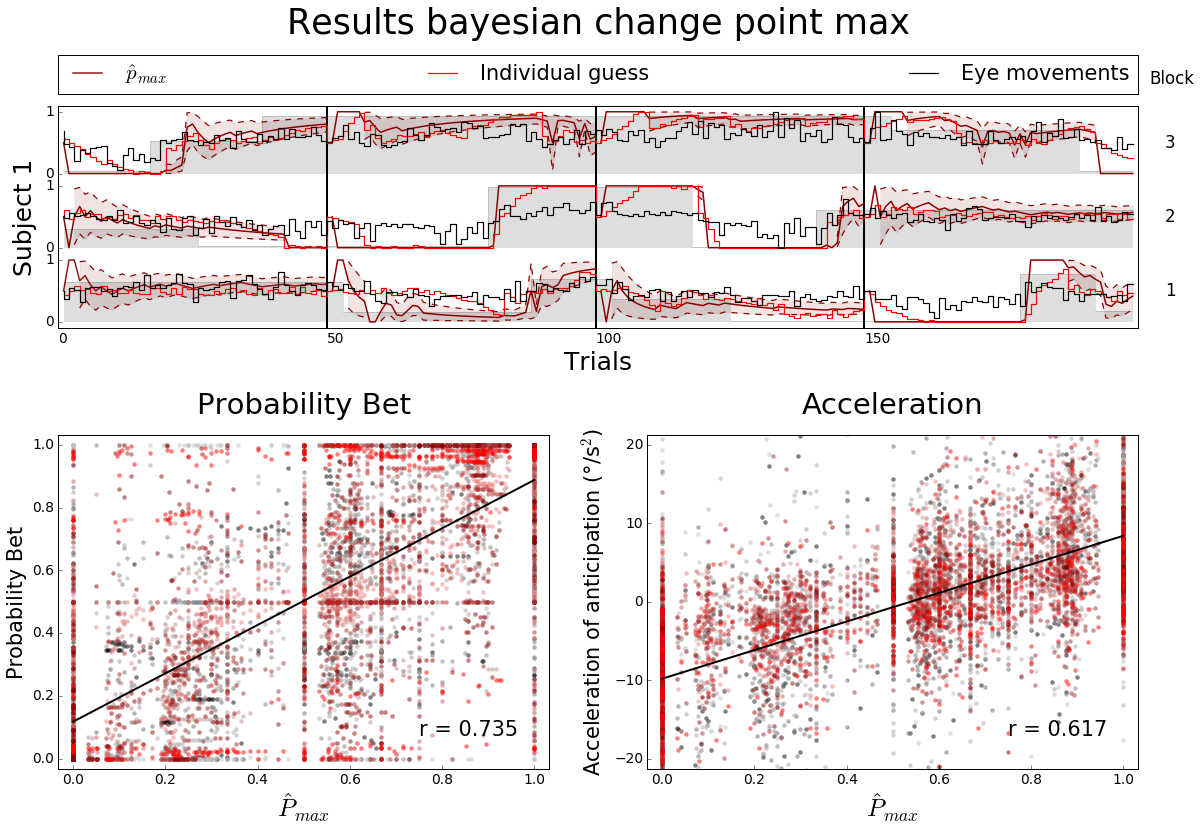
\includegraphics[width=1\linewidth]{results_bayesianchangepoint_m}
\end{center}
\caption{\emph{Bayesian change point model} \textbf{(A)} 
\textbf{(B)} 
\textbf{(C)}  }
\label{fig:results_psycho}
\end{figure}
%-------------------------------------------------------------%

include the comparison with a control agent, the forgetful agent with time characteristics $\tau$

\subsection{Analyzing inter-individual differences}

By extracting the parameters for every subject we can expect to characterise inter individual differences. 

%-------------------------------------------------------------%
%: fig:results_psycho_inter
\begin{figure}%[b!]
%\begin{center} 
%    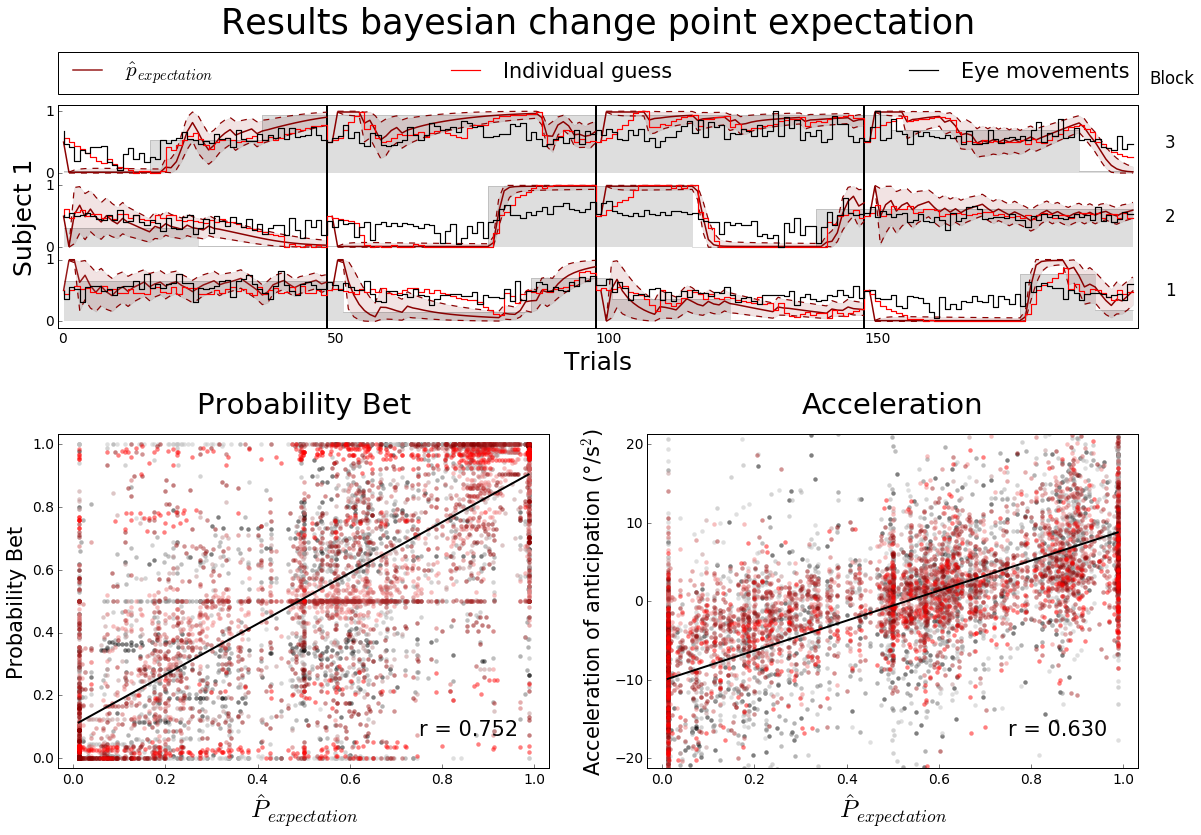
\includegraphics[width=1\linewidth]{results_bayesianchangepoint_e}
%    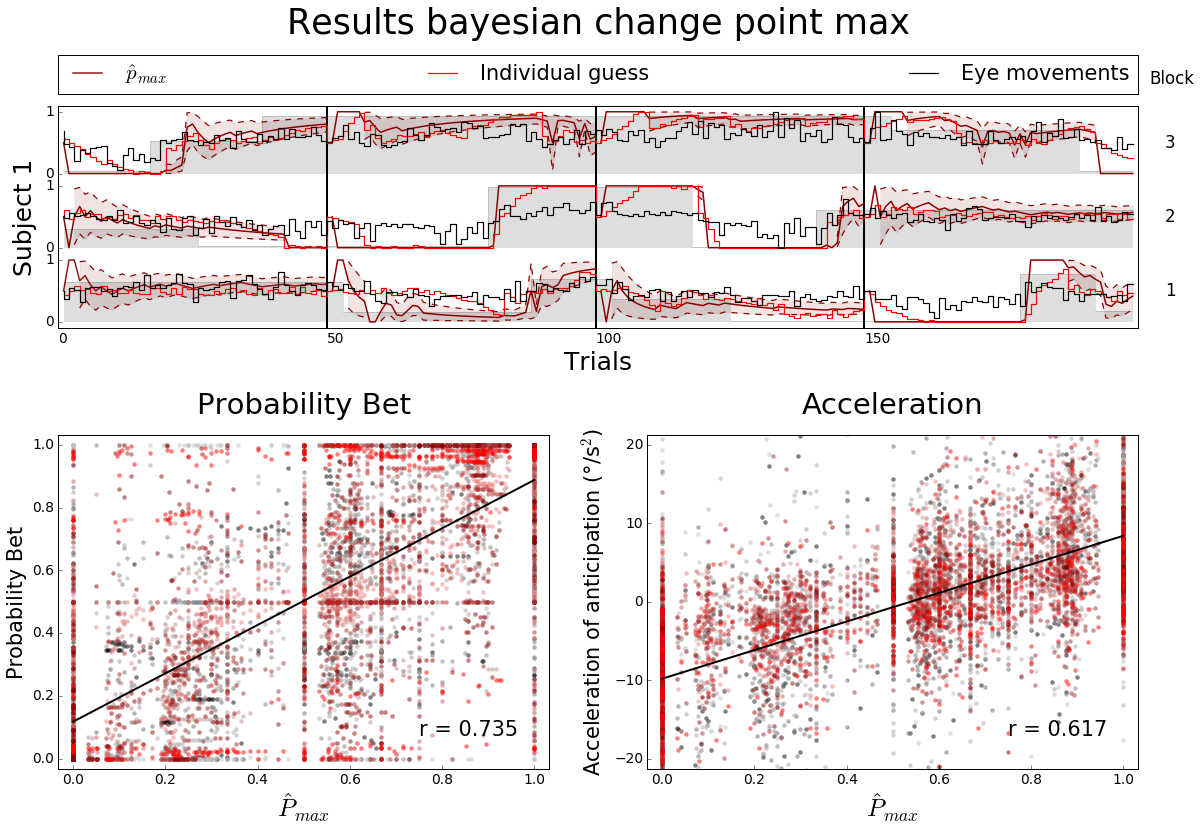
\includegraphics[width=1\linewidth]{results_bayesianchangepoint_m}
%\end{center}
\caption{\emph{Analyzing inter-individual differences} \textbf{(A)} 
\textbf{(B)} 
\textbf{(C)}  }
\label{fig:results_psycho_inter}
\end{figure}
%-------------------------------------------------------------%

There are a spectrum of individual choices between exploration and exploiting behaviors.



\section{Discussion}


\section{Conclusions}


\begin{itemize}\setlength{\itemsep}{0ex}
\item There is a strong correlation between the real probability and the value of the bet,

\item there is a stong correlation between the strength of anticipation and the probability of the process,

\item we have developed a Bayesian model of an agent estimating the probability of changing points. This allows to dynamically infer the direction probability and directly compare model and human behaviour.

\end{itemize}

{\tiny
\printbibliography
}
%%%%%%%%%%%%%%%%%%%%%%%%%%%%%%%%
\end{document}%
